% ============================================================
% emergence-study: master version (no venue).
%
% this is the long, complete paper. each venue gets its own
% thin wrapper later (venues/), which \input-s the same sections.
% see README.md for how to compile & how to port.
% ============================================================

\documentclass[11pt]{article}

% ---------- switches (true / false) ----------
\newif\ifanonymous
\anonymousfalse   % \anonymoustrue hides name, affiliation, acknowledgments & self-identifying links (for blind review).

\newif\ifshownotes
\shownotestrue    % \shownotesfalse hides every \note{} & \anecdote{} placeholder (for submission).

% ============================================================
% preamble: packages & commands, shared by every version.
% (venue templates load many of these themselves; venue wrappers
% may skip this file & use only the "commands" part at the bottom.)
% ============================================================

\usepackage[T1]{fontenc}
\usepackage[utf8]{inputenc}
\usepackage{lmodern}
\usepackage{microtype}
\usepackage[letterpaper, margin=1in]{geometry}

\usepackage{amsmath, amssymb}
\usepackage{graphicx}
\usepackage{booktabs}
\usepackage{tabularx}
\usepackage{enumitem}
\usepackage[font=small, labelfont=bf]{caption}
\usepackage{subcaption}
\usepackage[dvipsnames]{xcolor}
\usepackage[numbers, sort&compress]{natbib}
\usepackage[hidelinks]{hyperref}

\graphicspath{{figures/}}

% ------------------------------------------------------------
% commands (used in the sections; keep these in every version)
% ------------------------------------------------------------

% a note to the author: shown while drafting, hidden for submission.
\newcommand{\note}[1]{\ifshownotes{\color{Magenta}\small[\textbf{note:} #1]}\fi}

% a placeholder for the author's own anecdote.
\newcommand{\anecdote}[1]{\ifshownotes\par\noindent{\color{Magenta}\small\fbox{\parbox{0.96\linewidth}{\textbf{anecdote (to write):} #1}}}\par\fi}

% text that names the author or links to their work; hidden when anonymous.
\newcommand{\identifying}[2]{\ifanonymous #2\else #1\fi}

% code & names from the system (kept in lowercase, as written).
\newcommand{\code}[1]{\texttt{#1}}

% the title of an interpretation (kept in lowercase, as the author writes them).
\newcommand{\work}[1]{\emph{#1}}

% the three parts of an interpretation, as written in its header.
\newenvironment{interpretation}[1]
  {\par\medskip\noindent\textbf{interpretation #1}\par\smallskip
   \begin{description}[leftmargin=1.2em, labelindent=0em, font=\normalfont\itshape, itemsep=0.25em]}
  {\end{description}\medskip}


% ---------- title ----------
\title{Software-Interpretations of an Everyday System:\\[0.2em]
\large Emergence, Instruction, and the Artist as Reader}

\ifanonymous
  \author{Anonymous Author(s)}
\else
  \author{Arjun Yadav\\[0.3em]
    \small Interactive Telecommunications Program (ITP), Tisch School of the Arts\\
    \small New York University, New York, NY, USA\\
    \small \href{mailto:ay3020@nyu.edu}{\texttt{ay3020@nyu.edu}}}
\fi

\date{}

\begin{document}

\maketitle

\begin{abstract}
Generative art has long borrowed emergence from abstract rule systems: cellular automata, flocking, or the simple forms and behaviours of Casey Reas's \emph{Process Compendium}. Their rules are elegant, but arbitrary: they are chosen for what they produce, not for what they are about. This paper presents \emph{emergence-study}, an artwork and software system whose rules are instead drawn from the rhythms of everyday life. Beings in a simulated world are born, age, keep daily routines between places, stay, have children and die; how busy, how energetic and how long-lived they are depends on their age, with noise. The system itself is never shown. What is shown are \emph{software-interpretations}: each begins as a thought, written in English from the artist's lived experience, and is realised as an algorithm that reads selected data from the system and draws it. Every interpretation is documented in three parts, \emph{thought}, \emph{expression} and \emph{parameters}, a structure that extends the instruction-based practices of Sol LeWitt and Yoko Ono to a running simulation. I describe the base system in full, the interpretation method, and six interpretations made with it. I also report how the base system was revised after measurement, and show that the rules of the ground, not only the choices of the reader, decide what an interpretation can reveal. The work argues that a system built from everyday life lets one set of rules hold many readings that are at once personal and grounded, and it offers the three-part interpretation as a reusable, legible format for artists working with simulations.
\end{abstract}

\noindent\textbf{Keywords:} emergence, generative art, instruction art, agent-based simulation, software art, everyday life, process art, data representation.


\section{Introduction}
\label{sec:introduction}

In \emph{Dynamics of Complex Systems}, Yaneer Bar-Yam describes \emph{emergent complexity}: a system composed of simple parts whose collective behaviour is complex~\cite{baryam1997}. The outcome of such a system cannot be determined by studying its parts on their own. Snowflakes are a familiar example: each grows outward from its centre by a small set of local rules, yet the order in which those rules act, and the way the result of one rule shapes the conditions for the next, produce dendrites that are never quite alike~\cite{snowflake2022}. A social group is a closer one. There are rules between each pair of people within it, and rules for the group as a whole, and how these interact under changing conditions is very hard to predict.

For artists, this has been a productive idea for more than half a century. Systems art, process art and generative art all take, in different ways, the position that an artist can author the conditions from which a work emerges rather than the work itself~\cite{burnham1968, galanter2003, boden2009}. In computational practice, the canonical demonstrations of emergence are cellular automata~\cite{wolfram2002, gardner1970}, flocking~\cite{reynolds1987}, and, closest to this work, Casey Reas's \emph{Process Compendium}, in which simple \emph{forms} (a circle, a line) are given simple \emph{behaviours} (move in a straight line, change direction when touching another element), and what is exhibited is not the elements but drawings made from their relationships~\cite{reas2010, reasgithub}.

These systems share a quality that this paper takes as its starting point: their rules are \emph{arbitrary}. They are elegant and productive, but they are chosen for the forms they generate, not because they are about anything in particular. A rule such as ``a cell with two equal neighbours turns on'' has no referent; it is a means. This is not a flaw in those works, which are about form and process. It does, however, leave open a question that motivates this one: what happens to emergence as an artistic material when the rules themselves are drawn from life?

This paper presents \emph{emergence-study}, an ongoing artwork and software system that takes that question literally. Its rules are drawn from the motions and physical constraints of everyday life, loosely inspired by the daily movement of people in New York. A \emph{world} contains \emph{places}. A \emph{population} of \emph{beings} is born, sustained and killed by the world over \emph{time}. Beings express life through \emph{movement}, which is governed by a \emph{schedule}: a daily routine of places they frequent. Both the schedule and the movement depend on \emph{age}; the closer a being is to its twenties, for example, the busier its day is likely to be. Every such rule carries noise, so that the unlikely (a busy sixty-year-old, a frail twenty-year-old) is possible but rare. The system is explicitly not representative of any real city. It is, as its documentation says, ``merely inspired by a tiny part of the multitude i / we live in.''

Crucially, the system is never shown. What a viewer sees is a \emph{software-interpretation}: a thought written in English, drawn from the artist's own experience, and then realised as an algorithm that selects data from the running system and represents it. One interpretation reads the system as threads of fate between beings born close to each other; another as ripples sent out when two beings meet; another as lines of separation drawn between neighbouring places. All of them run on the same world and the same rules.

\paragraph{Contributions.} This paper makes three contributions:
\begin{enumerate}[leftmargin=1.5em, itemsep=0.2em]
  \item \textbf{A base system of everyday rules} (Section~\ref{sec:system}): an agent-based world in which routines, ageing, energy, birth and death, rather than abstract local rules, are the source of emergence. It is described in full, with its equations, so that it can be rebuilt and reused.
  \item \textbf{The software-interpretation as a method} (Section~\ref{sec:method}): a three-part format (\emph{thought}, \emph{expression}, \emph{parameters}) through which an artist reads a running system. It situates software art within the lineage of instruction art~\cite{lewitt1967, ono1964}, while separating the reader of a system from its maker.
  \item \textbf{Six interpretations and a revision} (Sections~\ref{sec:interpretations} and~\ref{sec:revision}): six works made with the method, and a measured account of how revising the base system changed what any interpretation could show. The second is, I argue, a finding in its own right: the ground on which interpretations stand is not neutral.
\end{enumerate}

Section~\ref{sec:background} situates the work in the literatures of emergence, instruction and generative art, artificial life, and everyday life and mobility. Section~\ref{sec:discussion} discusses what everyday rules afford and what they do not, the authorship of interpretations, and the limits of the claims made here.

\anecdote{a short paragraph on where this began: the itp personal statement (2024), first year pulling in other directions, & finding the way back to this enquiry at the recurse center in summer 2026. reviewers at art venues respond well to a brief, honest origin; keep it to 3--4 sentences. (the quote from the statement could go here, or as an epigraph under the title.)}

\section{Background and Related Work}
\label{sec:background}

This work sits where four bodies of work meet: the science of emergence and complex systems; instruction-based and conceptual art; generative and software art, including art made with artificial life; and the study of everyday life and human mobility, from which its rules are drawn.

\subsection{Emergence and rule systems}

That ``more is different'', that the behaviour of a whole is not readily deduced from the behaviour of its parts, is a long-standing observation across the sciences~\cite{anderson1972, simon1962}. Bar-Yam's account of emergent complexity, which motivates this work, frames it as a property of systems of simple parts whose collective behaviour is complex~\cite{baryam1997}; Holland describes emergence as ``much coming from little'', and locates it in rule-governed systems whose interactions generate perpetual novelty~\cite{holland1998}.\note{check holland's exact wording & page.}

The simplest computational systems that exhibit it are one-dimensional cellular automata. A cell holds one of two states (0, dead, off; or 1, alive, on). A row of cells is given, and each next row is computed by a rule-set in which every cell reads its neighbours in the previous row. Wolfram's \emph{A New Kind of Science} catalogues the behaviour of every such elementary rule~\cite{wolfram2002}; Conway's Game of Life, its two-dimensional cousin, became the public face of emergence~\cite{gardner1970}.

What interests me in these systems, as an artist, is a property that is easy to overlook: the state of a cell does not have to be drawn as black or white. It can be represented in any way at all, and the same rule, run from the same starting row, yields visibly different patterns depending on how each state is drawn (Figure~\ref{fig:ca}). A rule-set, in other words, \emph{affords more than its representation}. This observation is the seed of the software-interpretation (Section~\ref{sec:method}).

\begin{figure}[t]
  \centering
  \begin{subfigure}[t]{0.32\linewidth}
    
\includegraphics[width=\linewidth]{ca-2}
    \caption{0 and 1 as white and black.}
  \end{subfigure}\hfill
  \begin{subfigure}[t]{0.32\linewidth}
    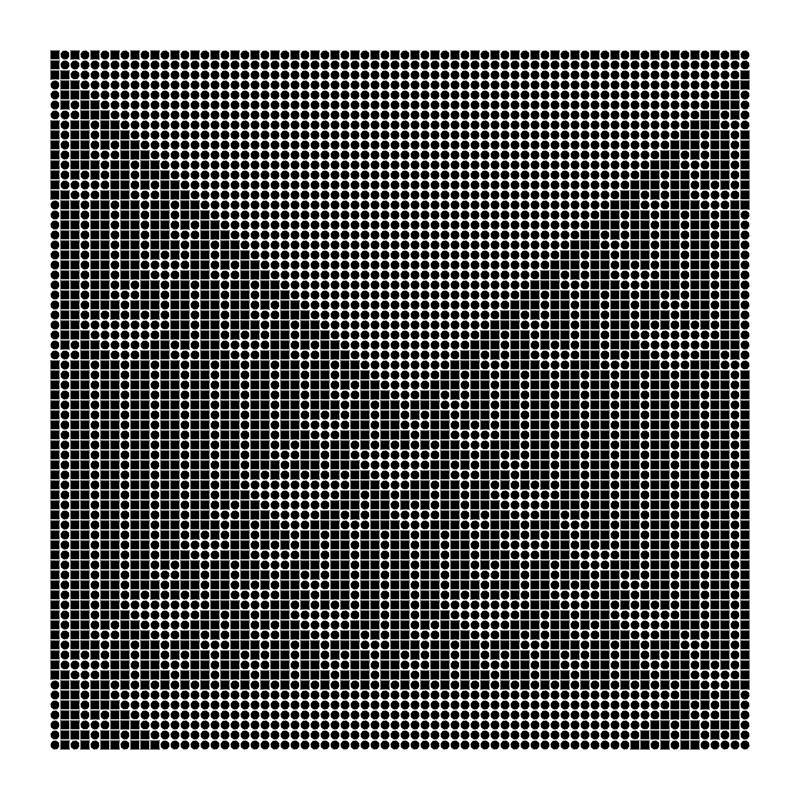
\includegraphics[width=\linewidth]{ca-3}
    \caption{0 as a square, 1 as a circle.}
  \end{subfigure}\hfill
  \begin{subfigure}[t]{0.32\linewidth}
    
\includegraphics[width=\linewidth]{ca-5}
    \caption{each state as a rotated line.}
  \end{subfigure}
  \caption{One elementary cellular automaton (rule~165, from a row of alternating cells), drawn three ways. The rule and the data are the same in each; only the representation differs, and with it the pattern one sees.}
  \label{fig:ca}
  \note{check: the rule & starting row for these images, & that all three were made by you (the talk credits one to wolfram).}
\end{figure}

\subsection{Instruction as artwork}

Conceptual art made the instruction itself the work~\cite{lewitt1967, lewitt1969}. Sol LeWitt wrote that ``the idea becomes a machine that makes the art''~\cite{lewitt1967}, and his wall drawings are sets of written instructions carried out by other people. \emph{Wall Drawing \#392} (1983), for instance, specifies a 12-inch grid over a black wall, with each square bisected by a vertical, horizontal or diagonal line, and leaves the direction of each line to the drafter~\cite{lewitt1983}. Two drafters following the same instruction produce wholly different walls; the online project \emph{Solving Sol} collects dozens of programmers' realisations of the same instructions in code~\cite{solvingsol}.

LeWitt's instructions are about form. Yoko Ono's are about experience. The instruction pieces collected in \emph{Grapefruit}~\cite{ono1964}, like George Brecht's event scores in \emph{Water Yam}~\cite{brecht1963}, are written in plain language and often ask for something to be imagined, noticed or lived rather than made. Hans Ulrich Obrist's long-running \emph{do it} project extends the format to hundreds of artists, each writing instructions that anyone may carry out~\cite{obrist2013}. Across all of these, the written instruction separates the work's \emph{idea} from its \emph{realisation}, and makes the gap between them the place where interpretation happens.

Vera Molnar's \emph{machine imaginaire}, the procedures she carried out by hand before she had access to a computer, shows how naturally this logic passed into computational art~\cite{molnar1975}. The software-interpretation keeps the plain-language instruction (the \emph{thought}) and its realisation (the \emph{expression}), but changes what is being instructed: not a drafter, but a reading of a system that is already running.

\subsection{Generative and software art}

Galanter defines generative art as any practice in which the artist uses a system, set into motion with some autonomy, that contributes to or results in a completed work~\cite{galanter2003}; Boden and Edmonds give a related taxonomy of generative and computer art~\cite{boden2009}. Burnham's earlier \emph{Systems Esthetics} had already argued that art was moving from objects to systems~\cite{burnham1968}.

The work most directly in conversation with this one is Reas's \emph{Process Compendium}~\cite{reas2010, reasgithub}. Reas defines \emph{elements} by pairing simple forms with simple behaviours, and then writes \emph{processes}: English-language descriptions of what to draw from the elements' interactions. Process~18, for instance, draws a quadrilateral between the end-points of each pair of elements that touch. The elements themselves are never shown. This separation, between a system and the drawing made from it, is the model for the software-interpretation. Reas has discussed the wider practice of code as a medium in \emph{Form+Code}~\cite{reas2010formcode} and, with Fry, built the Processing environment in which much of it happens~\cite{reasfry2007}; this work is written in its JavaScript descendant, p5.js~\cite{p5js}.

The difference I am concerned with is in the system that is read. Reas's elements are deliberately abstract, so that the processes are about form. In \emph{emergence-study}, the system is about something: the daily lives of beings. An interpretation of it can therefore be about something as well.

\subsection{Artificial life and agent-based models}

Artificial life set out to study ``life as it could be'' by synthesising life-like behaviour in software~\cite{langton1989}. Reynolds's boids showed that convincing flocks emerge from three local steering rules~\cite{reynolds1987}, and Whitelaw traces how artists took up such systems as a medium, a practice he calls \emph{metacreation}~\cite{whitelaw2004}. In the social sciences, agent-based models make a related move: Schelling showed that mild individual preferences about neighbours can produce stark segregation at the scale of a city~\cite{schelling1971}, and Epstein and Axtell's \emph{Sugarscape} grew trade, migration and inequality from agents with a few simple rules~\cite{epstein1996}.

\emph{emergence-study} borrows its form from these models: agents with traits, local rules, and a population that turns over. Its aim, however, is not to explain a social phenomenon, and its rules are not fitted to data. They are chosen so that they are recognisable as life, and so that they can carry an artist's reading.

\subsection{Everyday life and mobility}

Everyday life has its own theorists. Hägerstrand's time-geography describes each life as a path through space and time, held together by daily stations (home, work, others) and constrained by how far and how fast a body can move in a day~\cite{hagerstrand1970}; it is, in effect, the frame on which this system's routines are built. De Certeau reads walking in the city as an everyday practice that writes its own text over the planned city~\cite{decerteau1984}, and Lefebvre proposes a \emph{rhythmanalysis} of the repetitions that structure a day~\cite{lefebvre2004}. Jacobs's ``sidewalk ballet''~\cite{jacobs1961} and Whyte's filmed studies of plazas~\cite{whyte1980} attend to the same everyday movement at the scale of a street.

Empirical work has since found that human movement is highly regular: most people return again and again to a few places, and venture further only rarely~\cite{gonzalez2008, song2010}. Batty describes cities as systems of flows and networks rather than of places alone~\cite{batty2013}. These findings shaped the system's rules qualitatively (routines of a few nearby places, with the occasional long trip), though the system makes no claim to reproduce them quantitatively.

\subsection{Positioning}

Artistic data visualisation, as Vi{\'e}gas and Wattenberg describe it, uses the techniques of visualisation to make an argument or express a point of view rather than to support analysis~\cite{viegas2007}. A software-interpretation is close to this, with one difference: its data is not gathered from the world but generated by a system that the artist also made. The work therefore sits between three practices. Like instruction art, it begins with a written thought. Like generative art, it hands the realisation to a system. And like artistic data visualisation, it selects and represents data in order to say something. What it adds is a base system whose rules are themselves drawn from everyday life, so that the thought, the system and the drawing all refer to the same thing.

\section{The Base System}
\label{sec:system}

The base system is written in JavaScript with p5.js~\cite{p5js}, as two classes, \code{World} and \code{Being}, of about 900 lines together. It has no build step and no dependencies beyond p5.js. This section describes it in prose; the full equations are collected in Appendix~\ref{app:rules}. In summary:

\begin{quote}
There is a \emph{world}, and it consists of many \emph{places}. The world contains a \emph{population} of \emph{beings}, who are born, sustained and killed over \emph{time} by the world. Beings express life through \emph{movement}, and movement is governed by a \emph{schedule}. Both the schedule and the movement are governed by \emph{age}.
\end{quote}

\subsection{Design principles}

Four principles guided the system's design, and they explain most of its choices.

\begin{description}[leftmargin=1.2em, font=\normalfont\itshape]
  \item[Rules from life, not from form.] Every rule should be recognisable as something that happens in a life: keeping a routine, slowing down with age, having a child, dying. No rule exists only because it produces an interesting pattern.
  \item[Noise is intended.] Every trait and every age-dependent quantity is drawn with noise. The unlikely must be possible but not likely: a busy sixty-year-old, a frail twenty-year-old, a being who roams far from where it lives. Accordingly, the system is documented with ranges, not only averages (Figure~\ref{fig:graphs}).
  \item[No lockstep.] Nothing should happen to everyone at once. Each being's day starts at its own hour, and its plans change at its own moment, so the world moves continuously, calmly, and without global pulses.
  \item[Nothing is added that life does not suggest.] When a concept was tried and found to distort the system (Section~\ref{sec:revision} describes \emph{home}), it was removed rather than tuned.
\end{description}

\subsection{World, places and time}

The world is a rectangle of a given width and height. Its \emph{places} number one for every four beings at the start (at least two), and are laid out on a golden-angle, or sunflower, spiral~\cite{vogel1979} within a disc around the world's centre whose radius is 45\% of the world's shorter side. The spiral spreads places evenly without a grid, so that every place has a few neighbours at roughly the same distance, the \emph{place spacing}. A place has no fixed size: its radius grows with the crowd staying at it, so newcomers arrive at the edge of a crowd rather than at a point.

A day is always 24 hours, and beings live it the same way in every world. A separate parameter, the \emph{day length}, sets only how long a day lasts on screen (in seconds, at 60 frames per second); it is the world's playback speed. One day is also one year of a being's life: beings age by one year at every midnight. This compression lets a viewer watch whole lives, from birth to death, over an evening.

\subsection{Beings and their bodies}

A being is created with a position and an age. On creation it draws a set of personal traits, which play the role of a genome but are not inherited:
\begin{itemize}[leftmargin=1.5em, itemsep=0.1em]
  \item a \emph{maximum mass}, the size it grows to by about the age of eighteen;
  \item a \emph{walking pace}, a multiplier between 0.75 and 1.25;
  \item a \emph{range}, how far it is willing to travel between places, drawn log-normally so that most beings stay local and a few roam; and
  \item a \emph{vigor}, drawn log-normally around 1, which raises its energy and lengthens its life.
\end{itemize}
Its body then changes with age. \emph{Mass} grows asymptotically to its maximum; it determines only how large the being is drawn and how much room it takes up, not how fast it moves. \emph{Energy} is the product of two logistic curves, one rising through childhood (centred on age 12) and one falling through middle age (centred on 50), above a floor of one fifth, and scaled by vigor (Figure~\ref{fig:graphs}b). It climbs through childhood, plateaus through the twenties and thirties, is about 60\% of that plateau at fifty, and never falls to nothing. A being's \emph{speed} is proportional to its energy and its walking pace, and is measured in the world's own geography: at full energy, a being reaches a neighbouring place in about three-quarters of an hour.

\subsection{The routine}

Each being keeps a \emph{routine}: a closed loop of a few places it frequents, which it goes round every day, staying at each for a while. How many places it \emph{wishes} to visit, its \emph{busyness}, follows a bell curve over age that peaks at 25, between two and twelve places, with more noise further from the peak (Figure~\ref{fig:graphs}a). How many it actually \emph{gets} depends on its body and on distance.

A routine is built as follows. It begins at the place nearest to the being. Each next place is chosen near the last, with a likelihood that falls off exponentially with distance at the being's own range. A place is added only if there is still time in the day to get there, stay at least an hour, and get back round to the first place, so that the loop always closes within 24 hours; places that also leave room for the remaining wished-for stops are preferred. The loop is then laid out over the day from the being's own \emph{day start}, a random moment unique to it. Each slot of the schedule lasts as long as the trip to its place plus a minimum stay of one hour, and spare time is split into random shares across the stays, so that stays end at any moment rather than on the hour. If a slower body cannot fit the whole loop, its last places are dropped; a being with only one place stays there all day.

Every frame, a being checks which slot of its schedule the world's clock falls in. If that slot names a different place, it leaves for it, in a straight line, even if it had not yet arrived where it was going. On arrival it stays until the schedule says otherwise.

There is no \emph{home}. A new routine starts from the place nearest to wherever the being is, so the places a being frequents can change, and over many years it may drift from one neighbourhood to another. Routines change at birthdays: always for young children (ages 2--6), with even odds for ages 7--60, and with a one-in-four chance after 60; otherwise the same places are re-timed for the body's new pace. New plans are taken up only at the being's own day start, so nobody re-plans in lockstep at midnight. Beings under two do not move.

\subsection{Birth and death}

The world keeps its population near its starting size. Once a day, at a randomly chosen hour, if the population is above 95\% of its starting size, each being dies with a probability that rises with the cube of its age, above a small floor, and is scaled by the square of its frailty (the inverse of its vigor; Figure~\ref{fig:graphs}c). The chance is about 0.1\% at 20, 1.5\% at 50, 6\% at 80 and 12\% at 100. Whenever the population is below its starting size, beings aged 18--45 may reproduce with a neighbour of the same ages, with a probability that peaks in the late twenties; each pair has at most one child per round, and the newborn appears between its parents, wherever they happen to be.

\subsection{What the system does}

\begin{figure}[t]
  \centering
  \begin{subfigure}[t]{0.49\linewidth}
    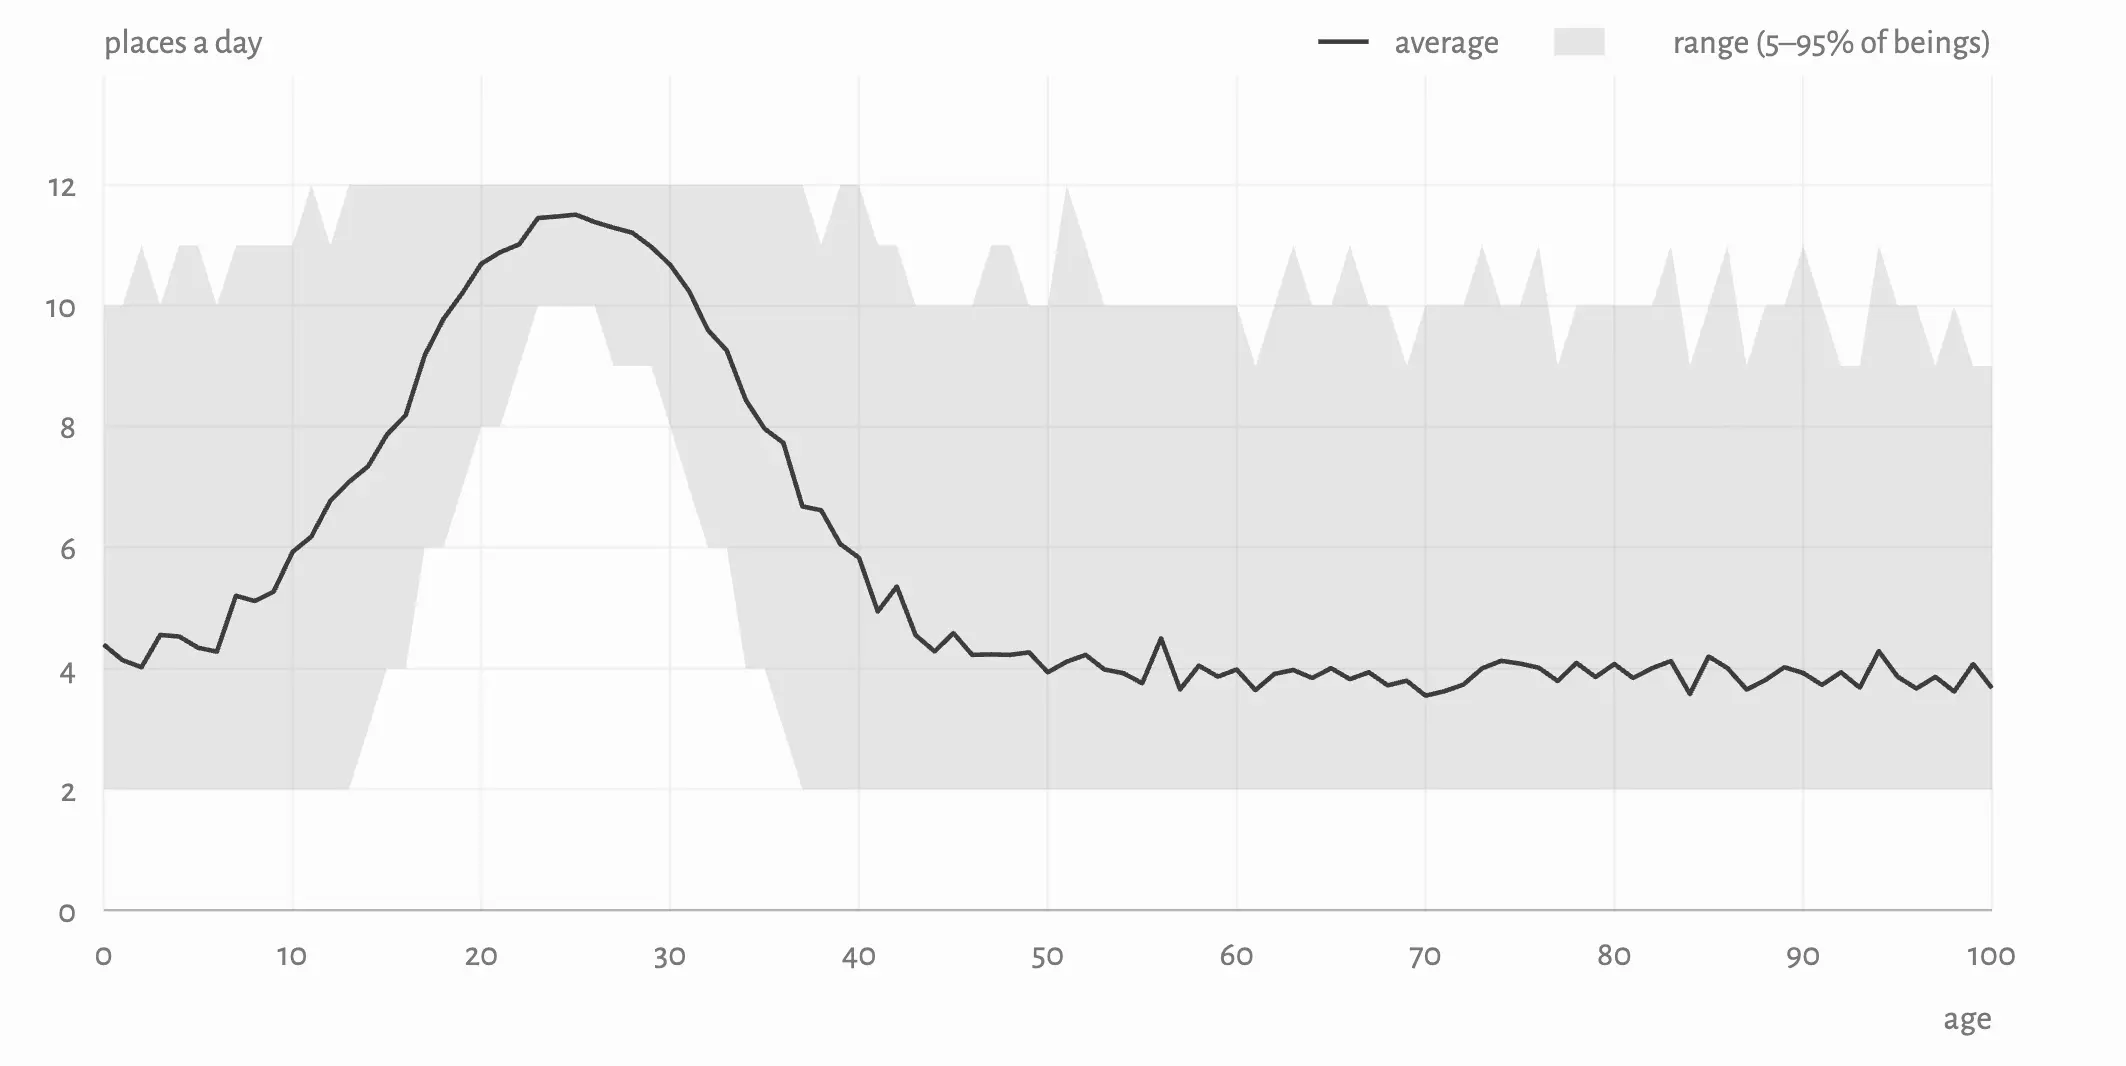
\includegraphics[width=\linewidth]{graph-busyness}
    \caption{Busyness (places wished for), over age: a bell curve peaking at 25, with wider noise away from the peak.}
  \end{subfigure}\hfill
  \begin{subfigure}[t]{0.49\linewidth}
    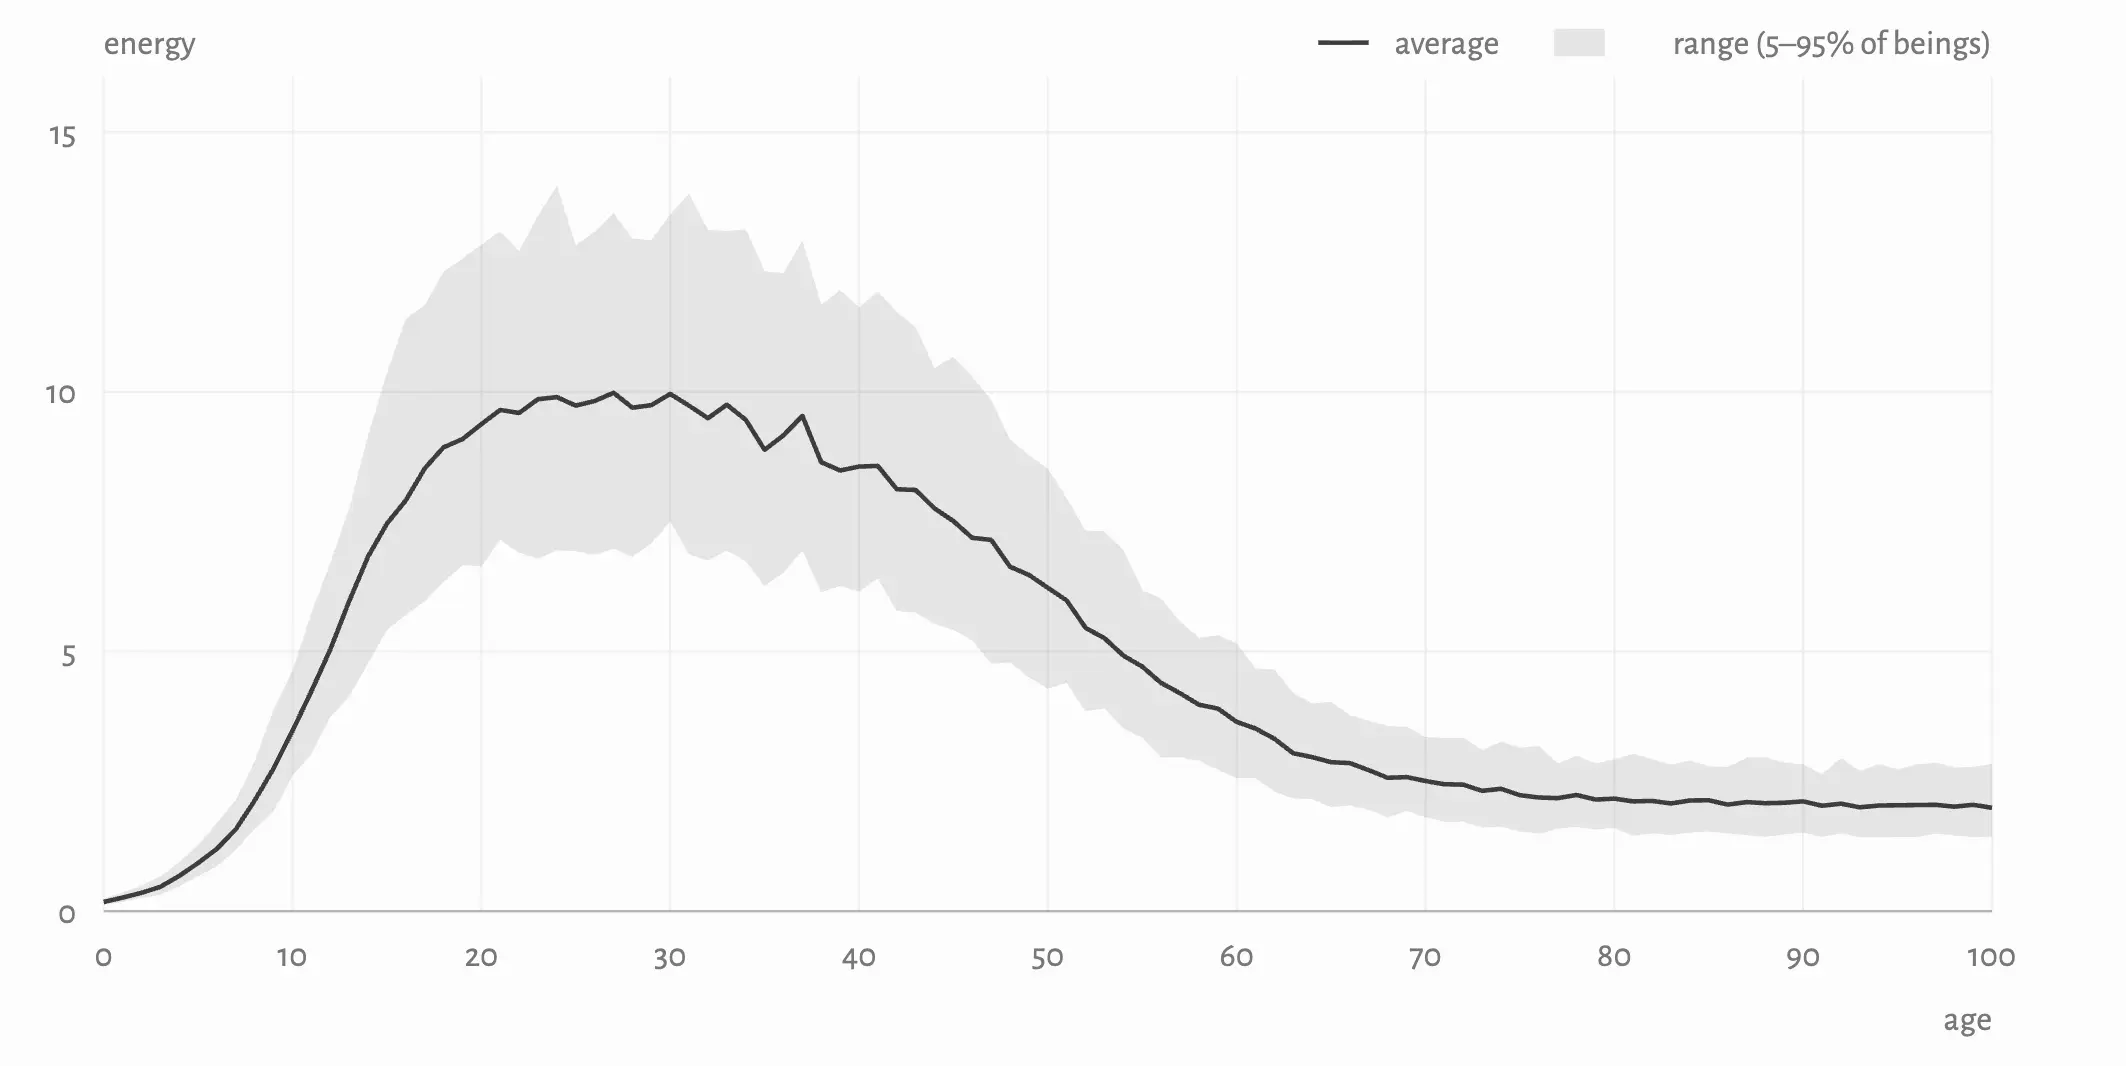
\includegraphics[width=\linewidth]{graph-energy}
    \caption{Energy, over age: two logistic curves multiplied, above a floor, scaled by log-normal vigor.}
  \end{subfigure}\\[0.6em]
  \begin{subfigure}[t]{0.49\linewidth}
    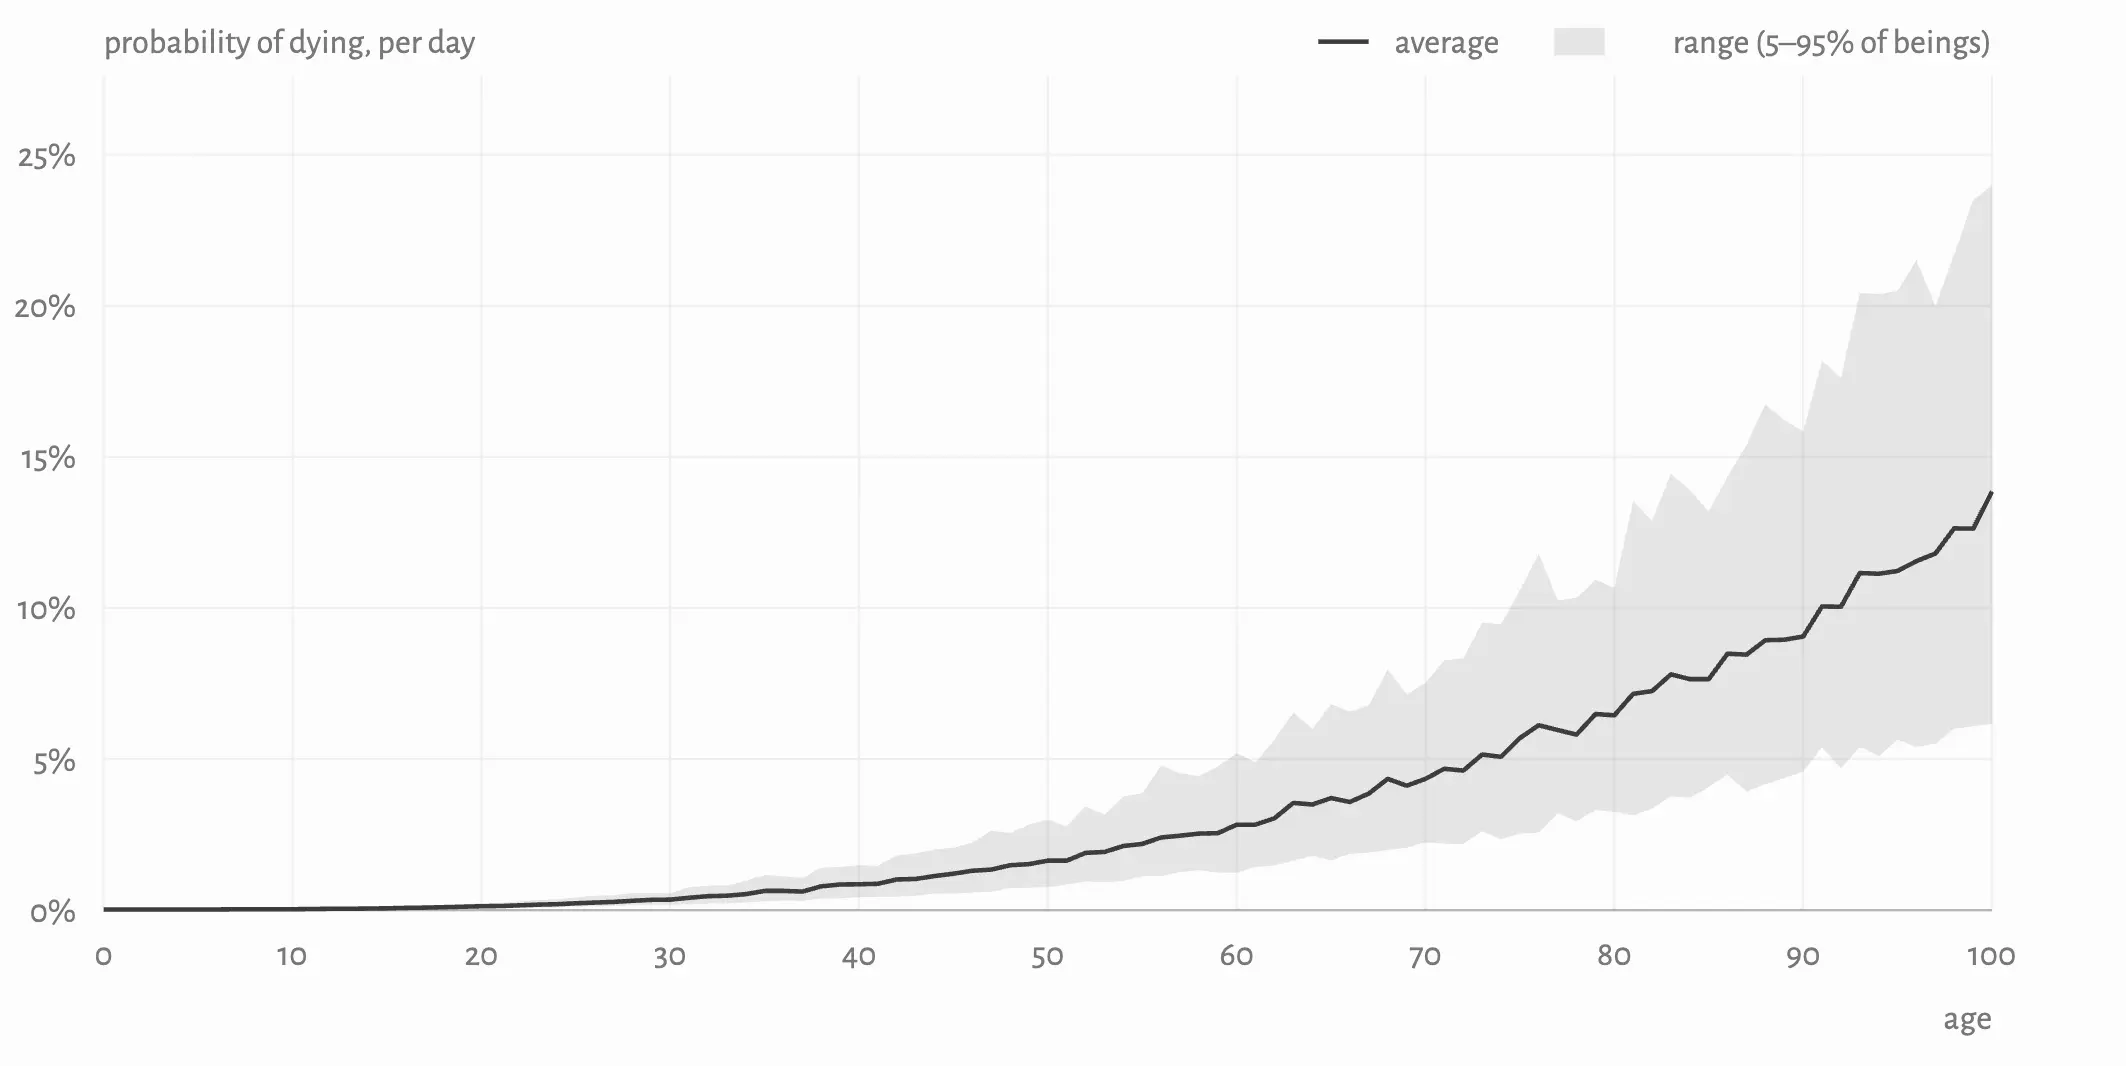
\includegraphics[width=\linewidth]{graph-dying}
    \caption{Probability of dying on a given day, over age: a cubic curve above a small floor, scaled by frailty squared.}
  \end{subfigure}\hfill
  \begin{subfigure}[t]{0.49\linewidth}
    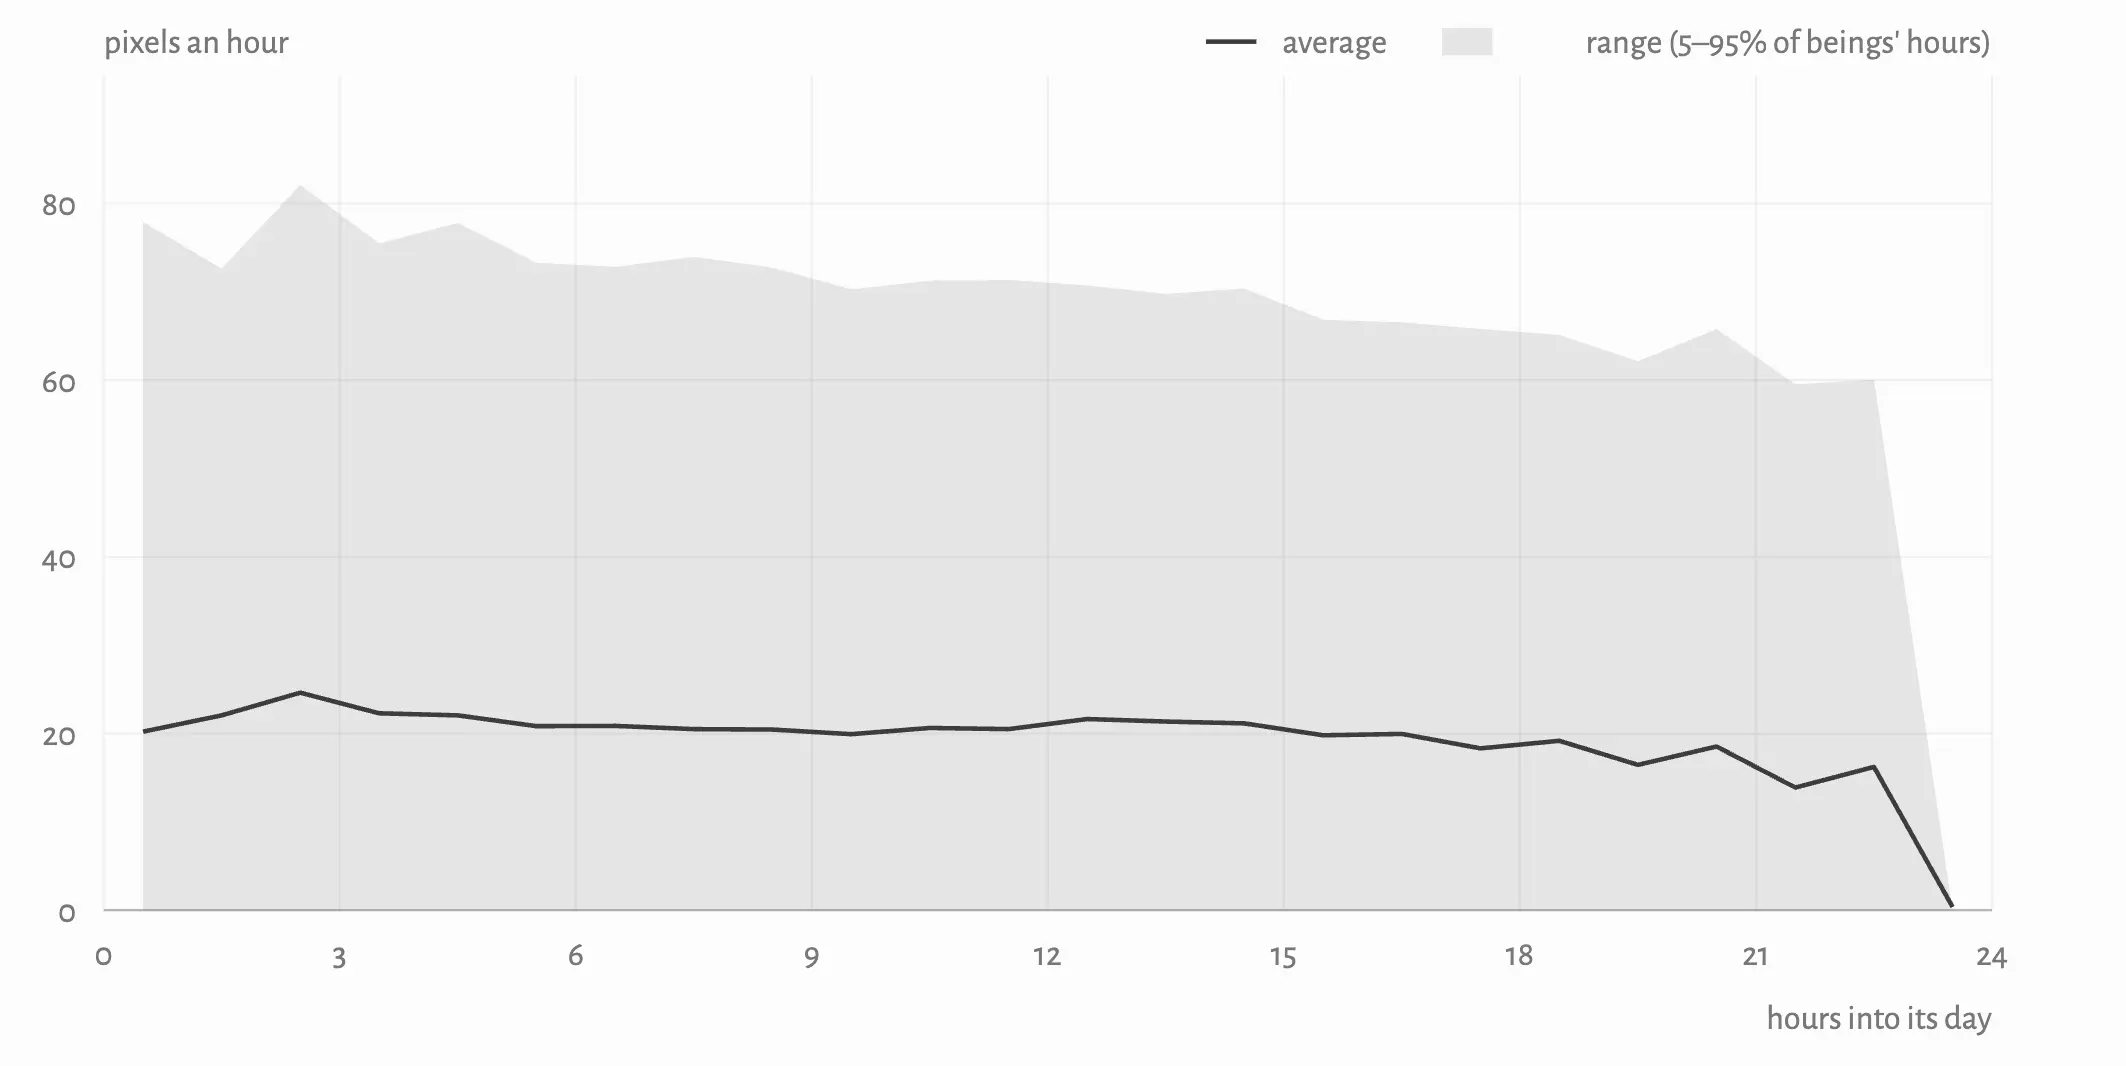
\includegraphics[width=\linewidth]{graph-movement}
    \caption{Pixels travelled in each hour of a being's own day. No equation: it emerges from the schedules.}
  \end{subfigure}\\[0.6em]
  \begin{subfigure}[t]{0.7\linewidth}
    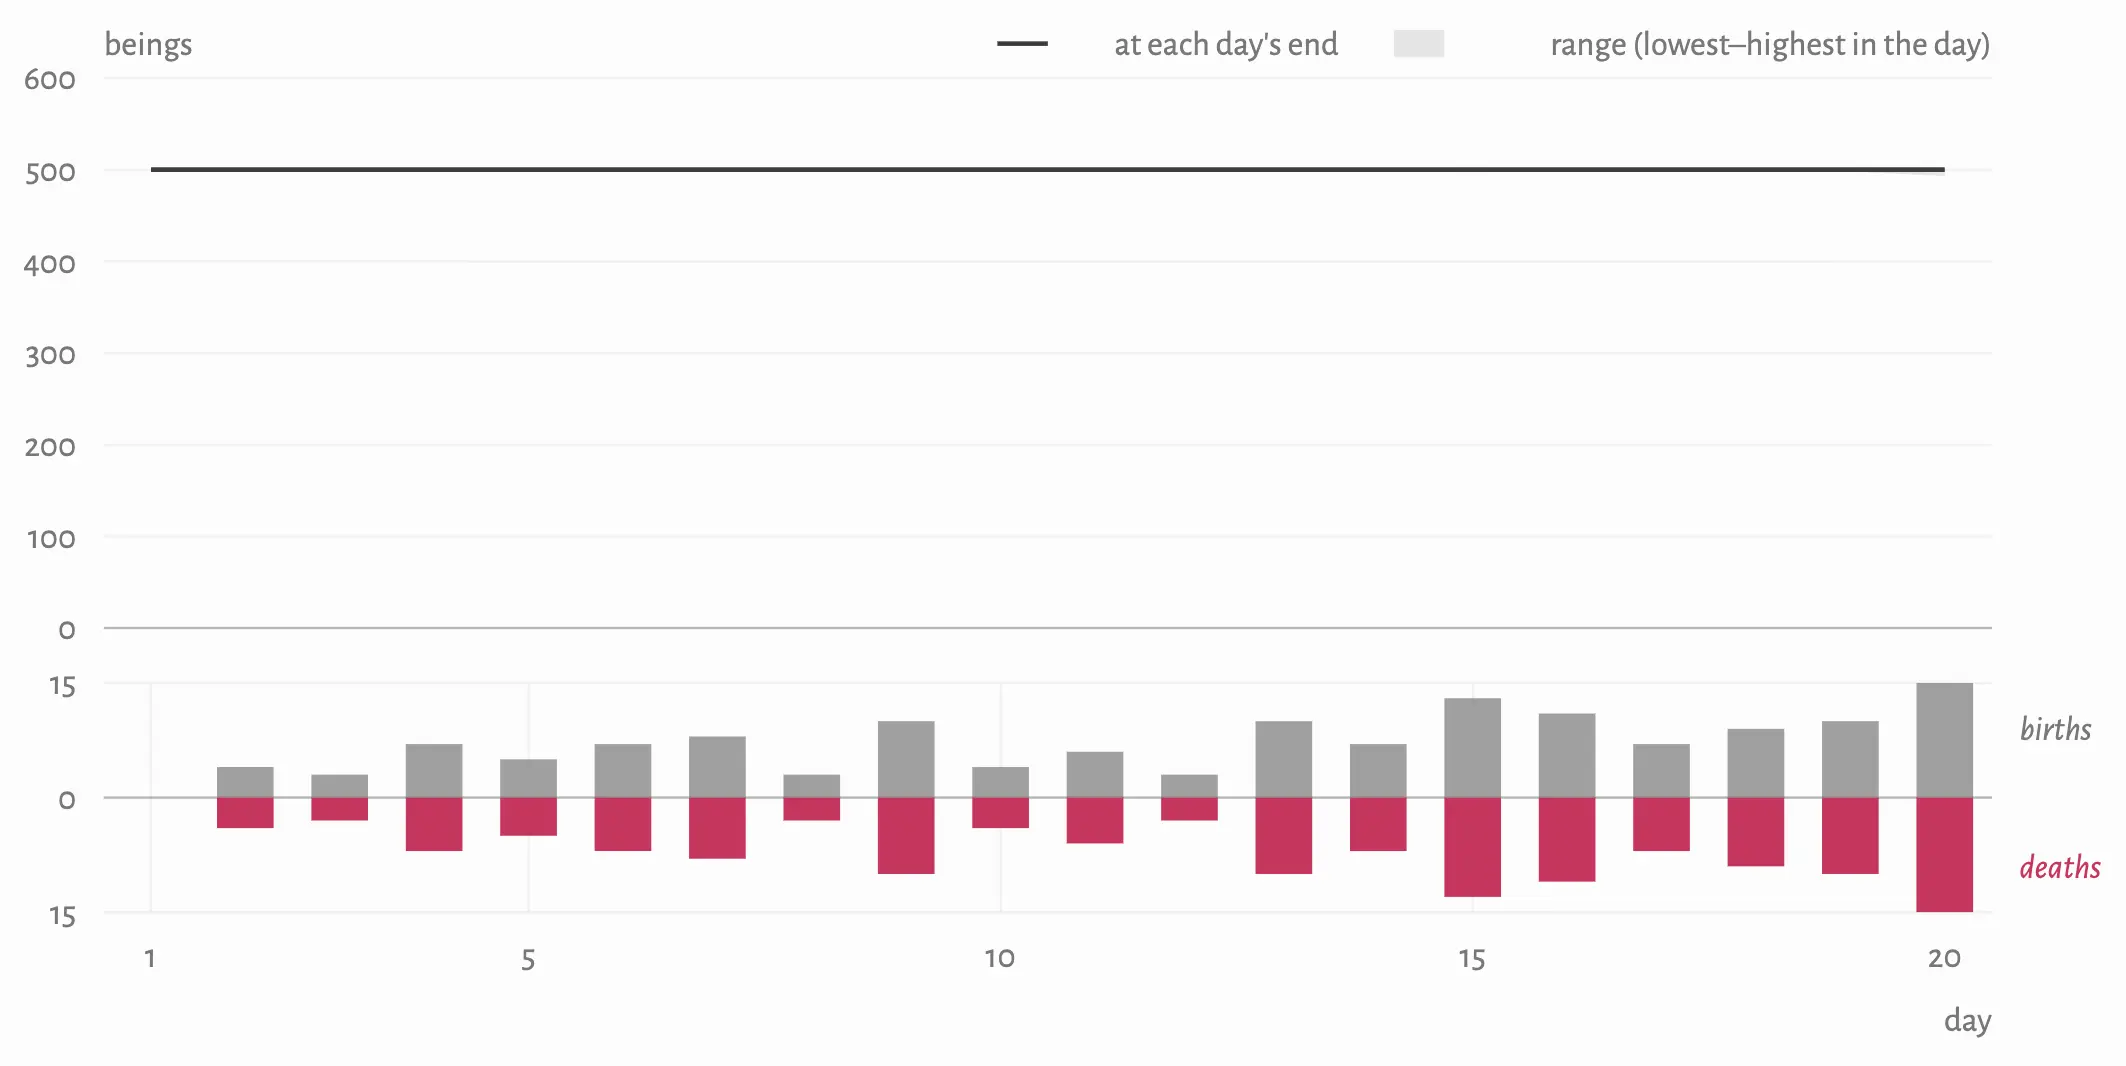
\includegraphics[width=\linewidth]{graph-population}
    \caption{Population at each day's end, with births and deaths: a feedback loop around a set point.}
  \end{subfigure}
  \caption{The base system, measured. Lines are averages; grey bands are ranges, because the system's noise is intended. (1440$\times$900 pixels, 500 beings, 20 days.)}
  \label{fig:graphs}
  \note{these graphs were measured before the day-length change; re-run \code{assets/cde/analysis/slide.html} & replace them before submission.}
\end{figure}

The system was measured headlessly, by running the real \code{World} and \code{Being} code outside the browser and instrumenting it (1440$\times$900 pixels, 500 beings; Appendix~\ref{app:reproducibility}). A few properties are worth noting, because no single rule specifies them.

\paragraph{A steady flow.} At any moment, about 28--35\% of beings are travelling (median 32\%), and this share is steady through the day, although no rule sets it. Departures are spread evenly in time: the busiest 1\% of moments account for only 1.9\% of departures. Distance travelled per hour of a being's own day is nearly flat (Figure~\ref{fig:graphs}d).

\paragraph{Lives that differ by age.} Places planned per day are about 11 for beings aged 18--35, 4 for 36--59 and 2 over 60; places actually reached are about 9.5 in the twenties and thirties, 5 in the forties, 3 in the fifties, and 2.5--2.8 after sixty. No being aged 18 or over spends a whole day at one place, and only 0.1\% of 18--45-year-olds reach no place on a given day. Most trips are short, but a few are long: about 2\% of trips cross more than five place spacings, and the longest nearly cross the world.

\paragraph{Lifespans that differ by vigor.} Median lifespan is about 62 for beings of low vigor, 70 for middling and 78 for high. Roughly 18.5\% of beings die before fifty, about 15\% live past ninety, and about 7\% reach a hundred.

\paragraph{A population that holds.} The population returns to its starting size within one or two frames of any death, and the age structure is stable over hundreds of days (median age about 32--36). Deaths match the death-chance formula within noise; every birth is to two neighbouring parents aged 18--45; and no being is a parent twice in a round.

\paragraph{Neighbourhoods without homes.} Without a home, routines spread across the world: after 400 days, at most 7 of 125 places go unused, the busiest place has three to four times the average crowd, and routines lean only slightly towards the centre (about 57\% of routine places lie in the inner half of the area, against 46\% at the start). Section~\ref{sec:revision} shows that this is not a given.
\note{the home / no-home numbers were measured with 5-hour days, before the day-length change. re-measure, or say so in the text.}

\subsection{What an interpretation can read}

An interpretation creates a world with four parameters (population, day length, maximum mass and a debug flag), and then reads it every frame. The world exposes its time of day (as an hour, \code{world.time}, and as a continuous clock), its places (each with a position and its current crowd), and its beings. Each being exposes its \code{age}, position (\code{pos}), \code{mass}, \code{energy}, \code{destination}, \code{busyness}, \code{schedule}, speed, and a query for its neighbours within a radius. Two internal properties are also read by some interpretations: a being's \code{state} (travelling or staying) and the \code{place} it is at or heading to.

This interface is deliberately narrow. An interpretation looks at the world but, by rule, never changes it; every interpretation therefore reads the \emph{same} system, and their differences are differences of reading.

\section{Software-Interpretations}
\label{sec:method}

A software-interpretation is the unit of the artwork. It is always written in English first, and then realised by an algorithm that the artist constructs. Every interpretation is documented, at the top of its source file, in three parts.

\begin{description}[leftmargin=1.2em, font=\normalfont\itshape]
  \item[Thought.] The core idea to express from the system, in plain language. A thought is written from the artist's lived experience, and is not derived from the system; it is a way of seeing that the artist brings to it. A thought should be legible to anyone, whether or not they read code.
  \item[Expression.] The technical account of how the thought is realised: which data are extracted from the system, how they are represented, and how the drawing develops over time (whether it accumulates, fades, or is cleared every frame). An expression should describe exactly what the code does.
  \item[Parameters.] The settings of the world in which the interpretation runs: population, day length and, where relevant, maximum mass. Some interpretations are computationally heavier than others, or need a denser or slower world to show what they look for, so the world is adjusted to the reading, but its rules never are.
\end{description}

Each interpretation also carries the date it was made.

\subsection{Thought and expression}

The split between thought and expression follows instruction art. In LeWitt's terms, the thought is the idea and the expression is its execution~\cite{lewitt1967}; in Ono's, the thought is the instruction, and much of its value lies in what it asks the reader to imagine~\cite{ono1964}. Writing the thought separately has two effects that I have found useful in practice.

First, it keeps the work honest. An expression can be checked against its thought: does this drawing actually say what the thought says? When it does not, either the expression changes or the thought is rewritten, and both changes are visible in the file's history. Second, it makes the work legible to people who will never read the code. In exhibition and in talks, an interpretation is introduced by its thought alone; the image is then read against it.

\subsection{The artist as reader}

In Reas's \emph{Process Compendium}, the artist authors the elements, their behaviours and the processes that draw them~\cite{reas2010}. In \emph{emergence-study} the same person authors both the base system and its interpretations, but in two distinct roles. As the maker of the system, I try to make rules that are true to life and that do not anticipate any particular reading. As its reader, I approach the running system with a thought, and look for the data that can carry it. The narrow interface of Section~\ref{sec:system}, through which an interpretation can read but not alter the world, is what keeps these roles apart.

This separation has a consequence worth stating plainly. The interpretations are not visualisations of the system, in the sense of showing it as it is. They are readings of it, each partial and each motivated. The same world, at the same moment, is at once a set of fated pairs, a field of passing encounters, a mesh, a pond of ripples, a fabric of ageing and a map of division. None of these readings is the system; all of them are drawn from it.

\subsection{An example}

The header of the third interpretation (Section~\ref{sec:mesh}) reads, in full:

\begin{quote}\small\ttfamily
interpretation \#3: all the world's a mesh.\\[0.4em]
thought:\\
all beings are connected to each other via an invisible mesh.\\[0.4em]
expression:\\
treat the position of each being as a vertex. generate a triangular-mesh by finding tuples close to each other, so that no point is inside a face. keep generating the mesh over time, as beings move.\\[0.4em]
parameters:\\
population: 1000,\\
day\_length: 24 (default).\\[0.4em]
24th july, 2026.
\end{quote}

The thought is a single sentence anyone can hold in mind. The expression names a technique (a Delaunay triangulation~\cite{delaunay1934}, computed with Delaunator~\cite{delaunator}) in plain terms, and states that the drawing accumulates. The parameters set a dense world, so that the mesh is fine.

\section{Six Interpretations}
\label{sec:interpretations}

This section presents the six interpretations made so far. Each is given with its thought and expression exactly as written in its source file, and its parameters as the code runs them. A short account of how it is realised follows, and then what it shows. The thoughts come from my own life; they are not drawn from any literature, and that is the point. Each runs full-screen in a browser; the stills shown here were captured from those runs.

% ------------------------------------------------------------
\subsection{born in pairs}
\label{sec:pairs}

\begin{interpretation}{\#1: born in pairs}
  \item[thought] beings are destined to be with someone that they were born close to (in proximity \& age). however, as they live out their lives, they may be close or separated in the world. thought is borrowed from the red thread of fate.\footnote{The red thread of fate is an East Asian folk belief, in which an invisible red cord ties together people who are destined to meet.\note{add a source for the red thread, if a venue asks for one; a book on chinese or japanese folklore is better than a website.}}
  \item[expression] draw a set of red lines between two beings that are `destined' to be together, over time. the closer they are to each other in space, the more red lines are drawn \& the stronger they are (in color \& density).
  \item[parameters] population: 200 (4 pairs shown); day length: 48.
\end{interpretation}

\paragraph{Realisation.} When the world is created, its beings are paired by how close they were born, in space (as a share of the world's diagonal) and in age (as a share of a hundred years), weighted equally: starting from one being, the chain repeatedly steps to the nearest remaining being, and consecutive beings in the chain are paired. Only the first four pairs are drawn. Every frame, each living pair is joined by a bundle of red lines: between two and ten of them, more when the pair is close, each thinner, paler and less saturated as the pair moves apart, and each jittered slightly by noise. The drawing accumulates. A pair's thread ends when either of them dies.

\paragraph{What it shows.} Because beings keep routines, one of a pair is often staying while the other travels. A line held at one end while its other end moves in a straight line sweeps out a triangle, and the image is built from these fans: deep red where the two were close, fading to pink and white where their days took them apart (Figure~\ref{fig:pairs}). The shape of each pair's drawing is, in effect, the shape of how their two routines overlapped over a lifetime.

\anecdote{why this thought: what made you think of the red thread, & of people born close to each other drifting apart or staying together.}

\begin{figure}[t]
  \centering
  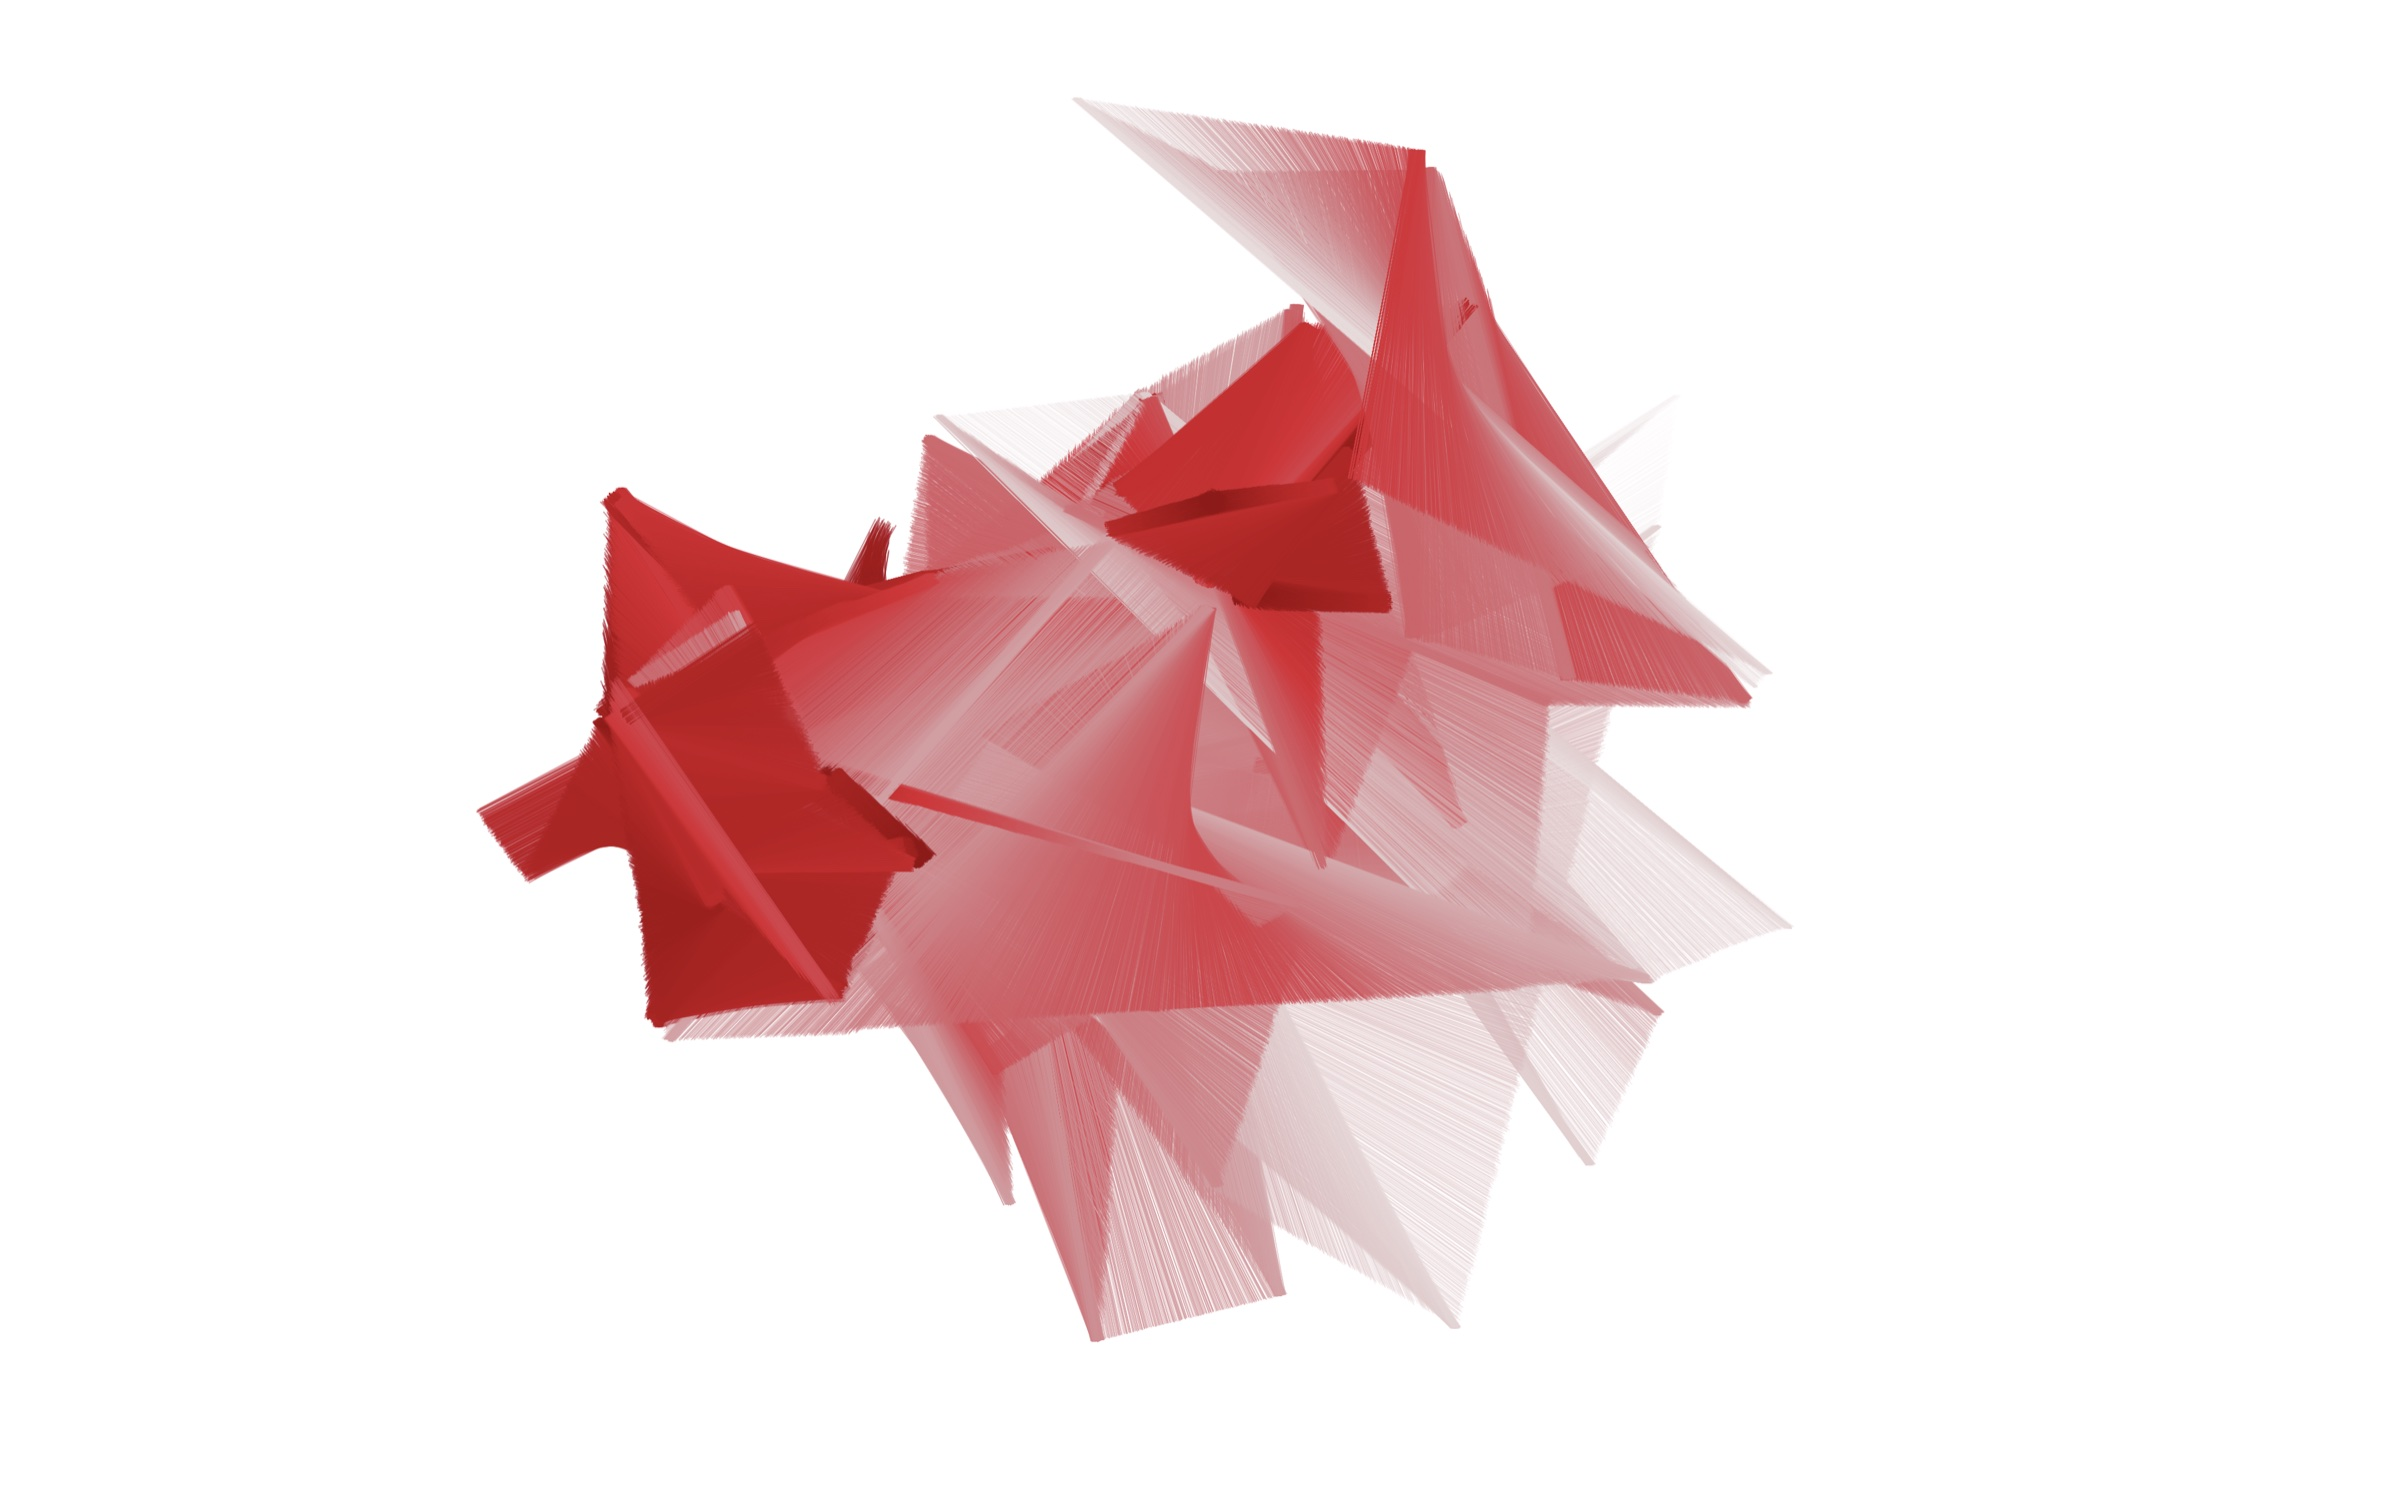
\includegraphics[width=0.85\linewidth]{interp-1}
  \caption{\work{born in pairs}: four pairs, over their lifetimes. Each fan is swept out by a thread held at one being's place while the other travels.}
  \label{fig:pairs}
\end{figure}

% ------------------------------------------------------------
\subsection{missed connections}
\label{sec:missed}

\begin{interpretation}{\#2: missed connections}
  \item[thought] we walk by so many people. when they are within a certain distance, we have a short window of time to connect with each other in physical-space, until we are distant again.
  \item[expression] draw a line from each being to other beings around them within a specific radius; while one of them is travelling. the closer they are, the thicker the line.
  \item[parameters] population: 1000; day\_length: 48; max\_mass: 6.
\end{interpretation}

\paragraph{Realisation.} Every frame, on a white ground that is cleared each time, each being looks for neighbours within three times its own size. A black line joins the two if at least one of them is travelling; beings staying together at a place are not passing each other, and are not joined. The line is thickest when the two are touching and thins to almost nothing at the edge of the radius.

\paragraph{What it shows.} This is the only interpretation that does not accumulate: it shows only the present. Lines appear as two beings approach, thicken as they pass, thin as they part and disappear, so every connection is visibly brief. Crowds at places stay unconnected unless someone is arriving or leaving through them, and the drawing is busiest on the routes between places, where travellers cross.

\anecdote{why this thought: a moment of walking past someone in new york, & the window closing.}

\note{there's no still of \#2 yet. add one (or a short sequence of three frames, since it's the only interpretation that's cleared every frame), as Figure~X.}

% ------------------------------------------------------------
\subsection{all the world's a mesh}
\label{sec:mesh}

\begin{interpretation}{\#3: all the world's a mesh}
  \item[thought] all beings are connected to each other via an invisible mesh.
  \item[expression] treat the position of each being as a vertex. generate a triangular-mesh by finding tuples close to each other, so that no point is inside a face. keep generating the mesh over time, as beings move.
  \item[parameters] population: 1000; day\_length: 24 (default).
\end{interpretation}

\paragraph{Realisation.} Every frame, the positions of all beings are triangulated (a Delaunay triangulation~\cite{delaunay1934, delaunator}) and every triangle is drawn with an almost transparent stroke, alternately black and white; the black-edged triangles are also filled with a nearly transparent white, slightly more opaque the smaller they are. The drawing accumulates over time.

\paragraph{What it shows.} The places are never drawn, but they appear (Figure~\ref{fig:mesh}). Where a crowd is staying, many vertices sit still at nearly the same point frame after frame, and the accumulated triangles meet there as stars. Between them, the routes between places are drawn as denser strands. The disc within which places lie becomes a dense, finely knit core, and beyond it, where few beings go, the mesh stretches into long, thin triangles reaching to the edges of the world. Over time, the mesh records not where beings are, but where they keep returning.

\anecdote{why this thought: what ``invisible mesh'' means to you in daily life.}

\begin{figure}[t]
  \centering
  \begin{subfigure}[t]{0.32\linewidth}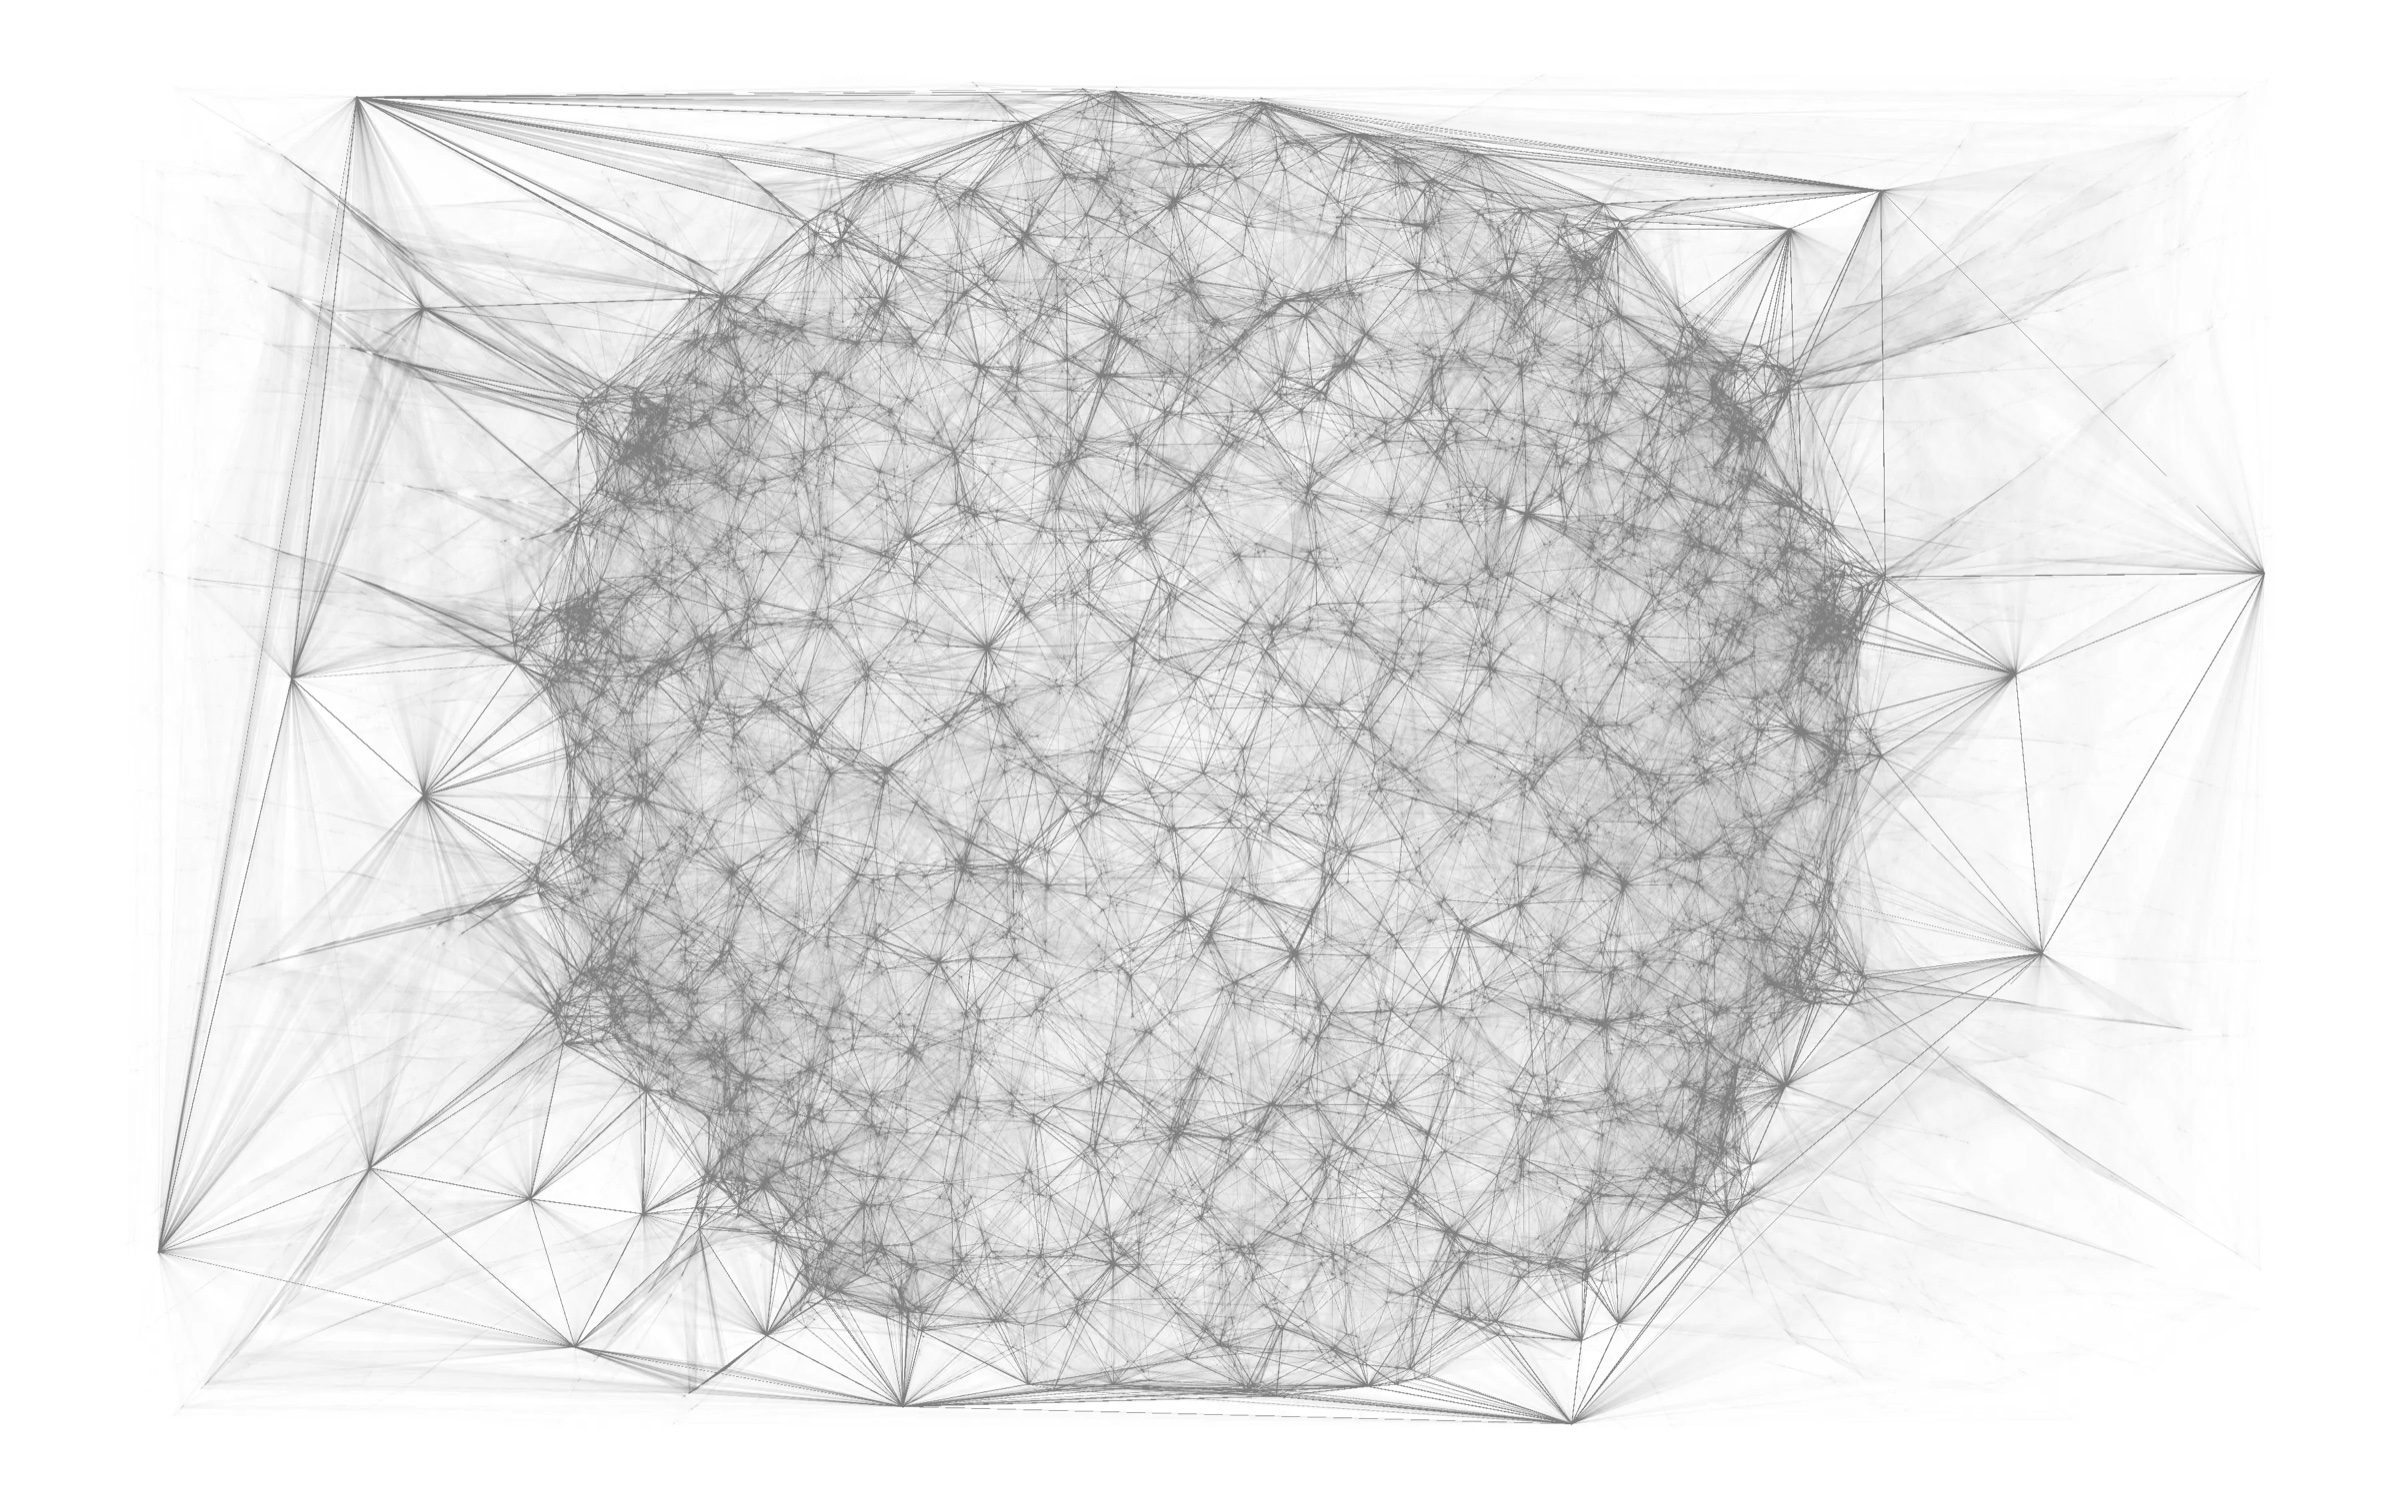
\includegraphics[width=\linewidth]{interp-3-1}\caption{}\end{subfigure}\hfill
  \begin{subfigure}[t]{0.32\linewidth}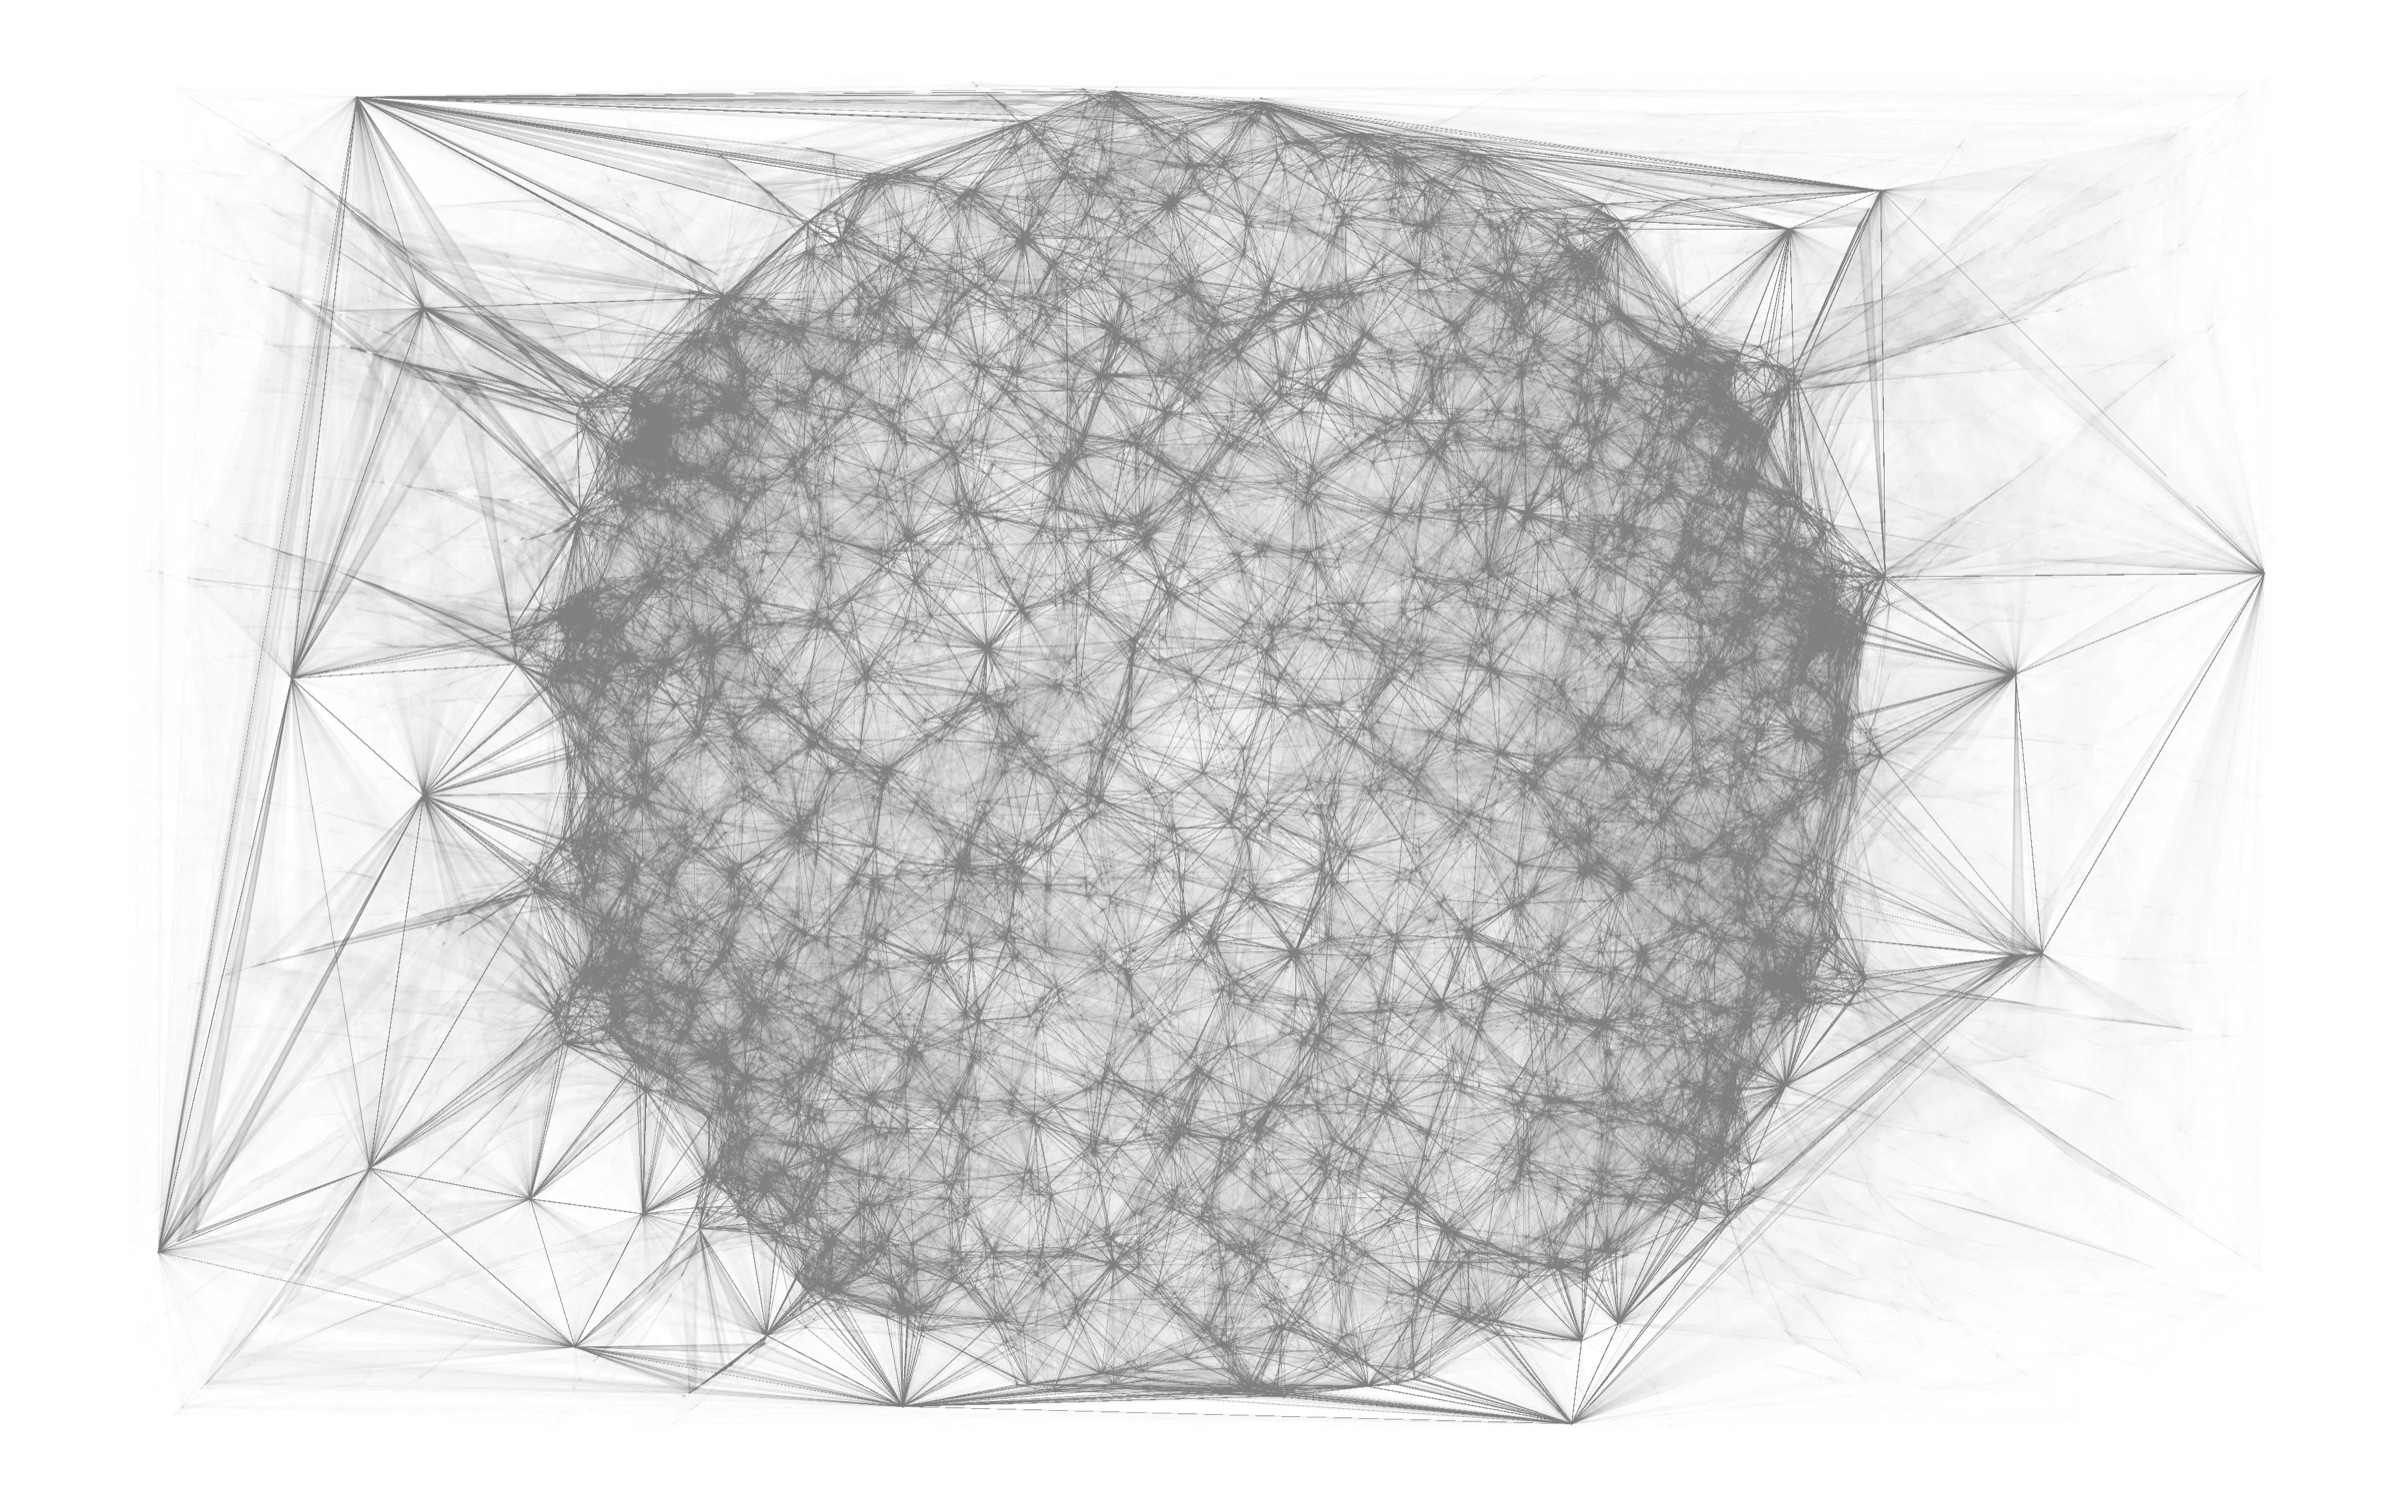
\includegraphics[width=\linewidth]{interp-3-2}\caption{}\end{subfigure}\hfill
  \begin{subfigure}[t]{0.32\linewidth}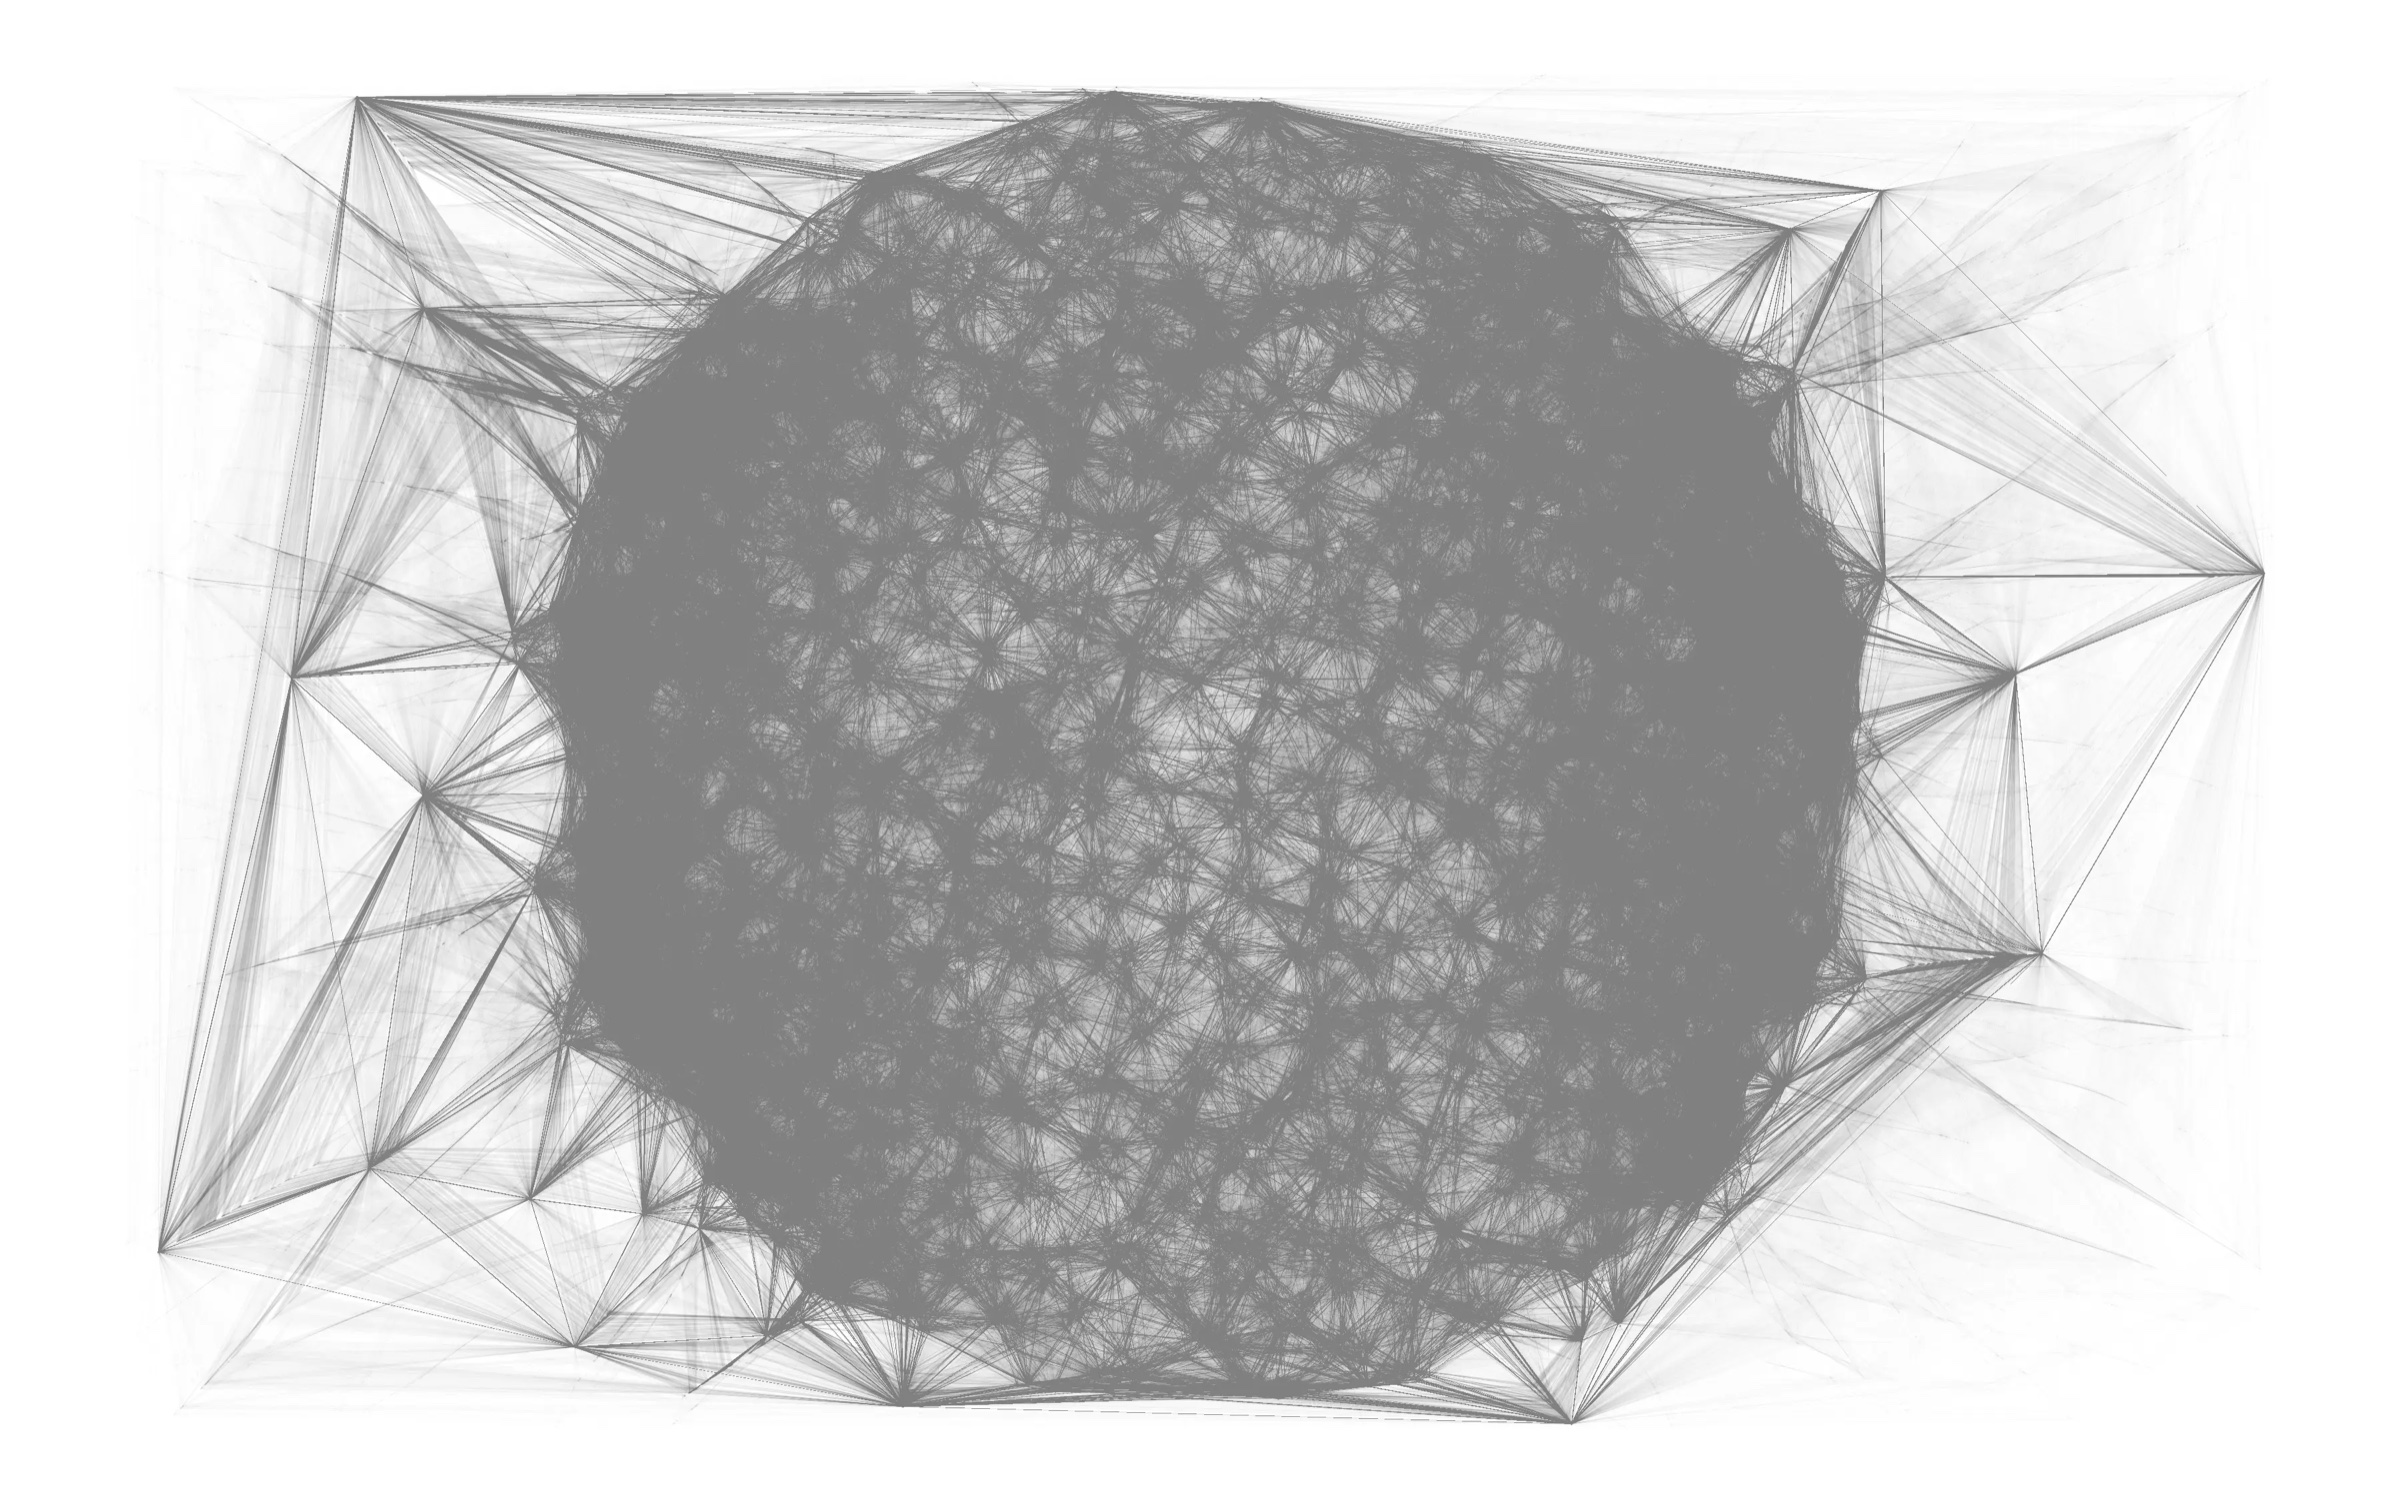
\includegraphics[width=\linewidth]{interp-3-3}\caption{}\end{subfigure}
  \caption{\work{all the world's a mesh}, at three points in time. The places, never drawn, appear as the stars of the mesh.}
  \label{fig:mesh}
  \note{check the order of the three images & what times they are from.}
\end{figure}

% ------------------------------------------------------------
\subsection{meetings are ripples}
\label{sec:ripples}

\begin{interpretation}{\#4: meetings are ripples}
  \item[thought] meeting people can be resounding. when two beings meet, a ripple is sent through space \& time; that may affect other beings.
  \item[expression] connect travelling beings close to each other with a black line. when two beings collide, send out a circular ripple expanding from the point of collision. the closer the beings are, the further the ripple goes. lay this out over time.
  \item[parameters] population: 500; day\_length: 48; max\_mass: 20.
\end{interpretation}

\paragraph{Realisation.} The ground is black and never cleared. A \emph{meeting} lasts from when two beings come within twice the maximum mass of each other until they part. At its closest moment, it sends out one ripple from the point between them: a ring of slightly jittered white points that expands by a pixel every frame and slowly fades. The closer the meeting, the further its ripple goes, from fifty pixels for a glancing pass to the width of the world for a collision. At most a hundred ripples exist at once, and none starts within twenty pixels of another, so many meetings pass without one. Meanwhile, every travelling being draws a very faint black line to one close neighbour.

\paragraph{What it shows.} The ripples accumulate into a luminous grey haze, brightest where meetings happen most, which is to say at and around places (Figure~\ref{fig:ripples}). The black lines, which would be invisible on black, become visible only where ripples have first lit the ground: travel is seen only where meetings have been. Where many beings pass, these lines carve a dark web through the haze.

\anecdote{why this thought: a meeting that was ``resounding'' for you.}

\begin{figure}[t]
  \centering
  \begin{subfigure}[t]{0.49\linewidth}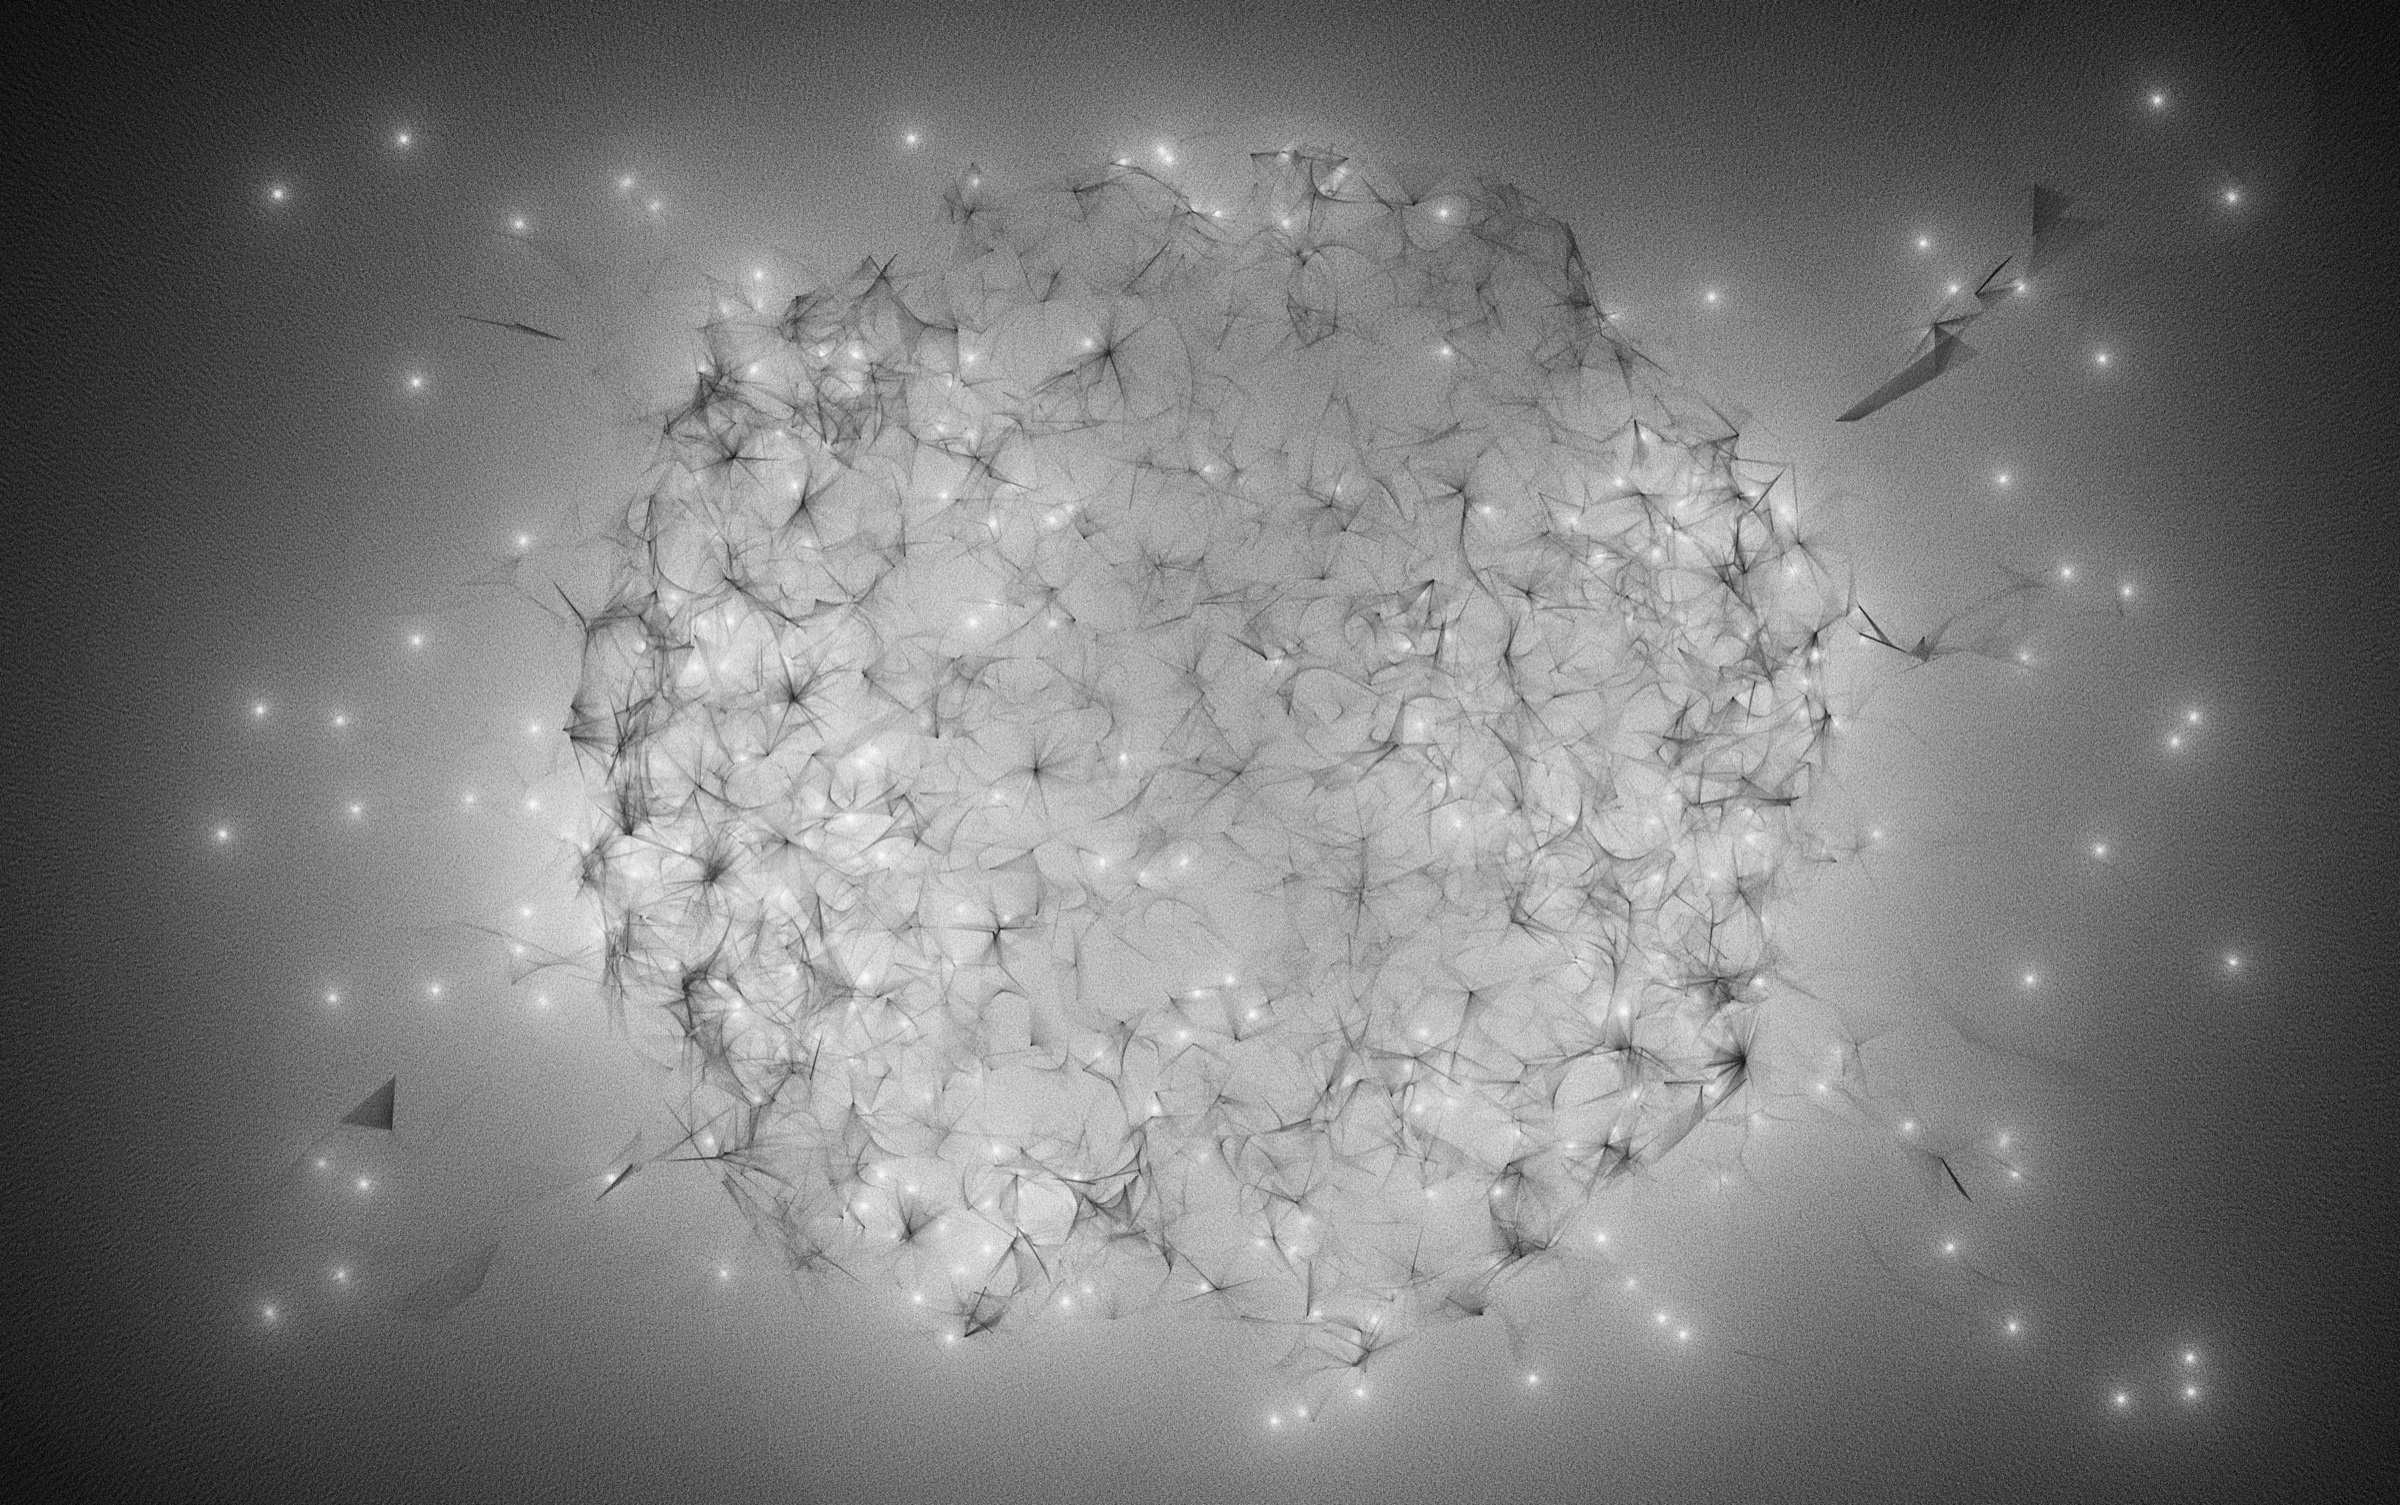
\includegraphics[width=\linewidth]{interp-4-1}\caption{}\end{subfigure}\hfill
  \begin{subfigure}[t]{0.49\linewidth}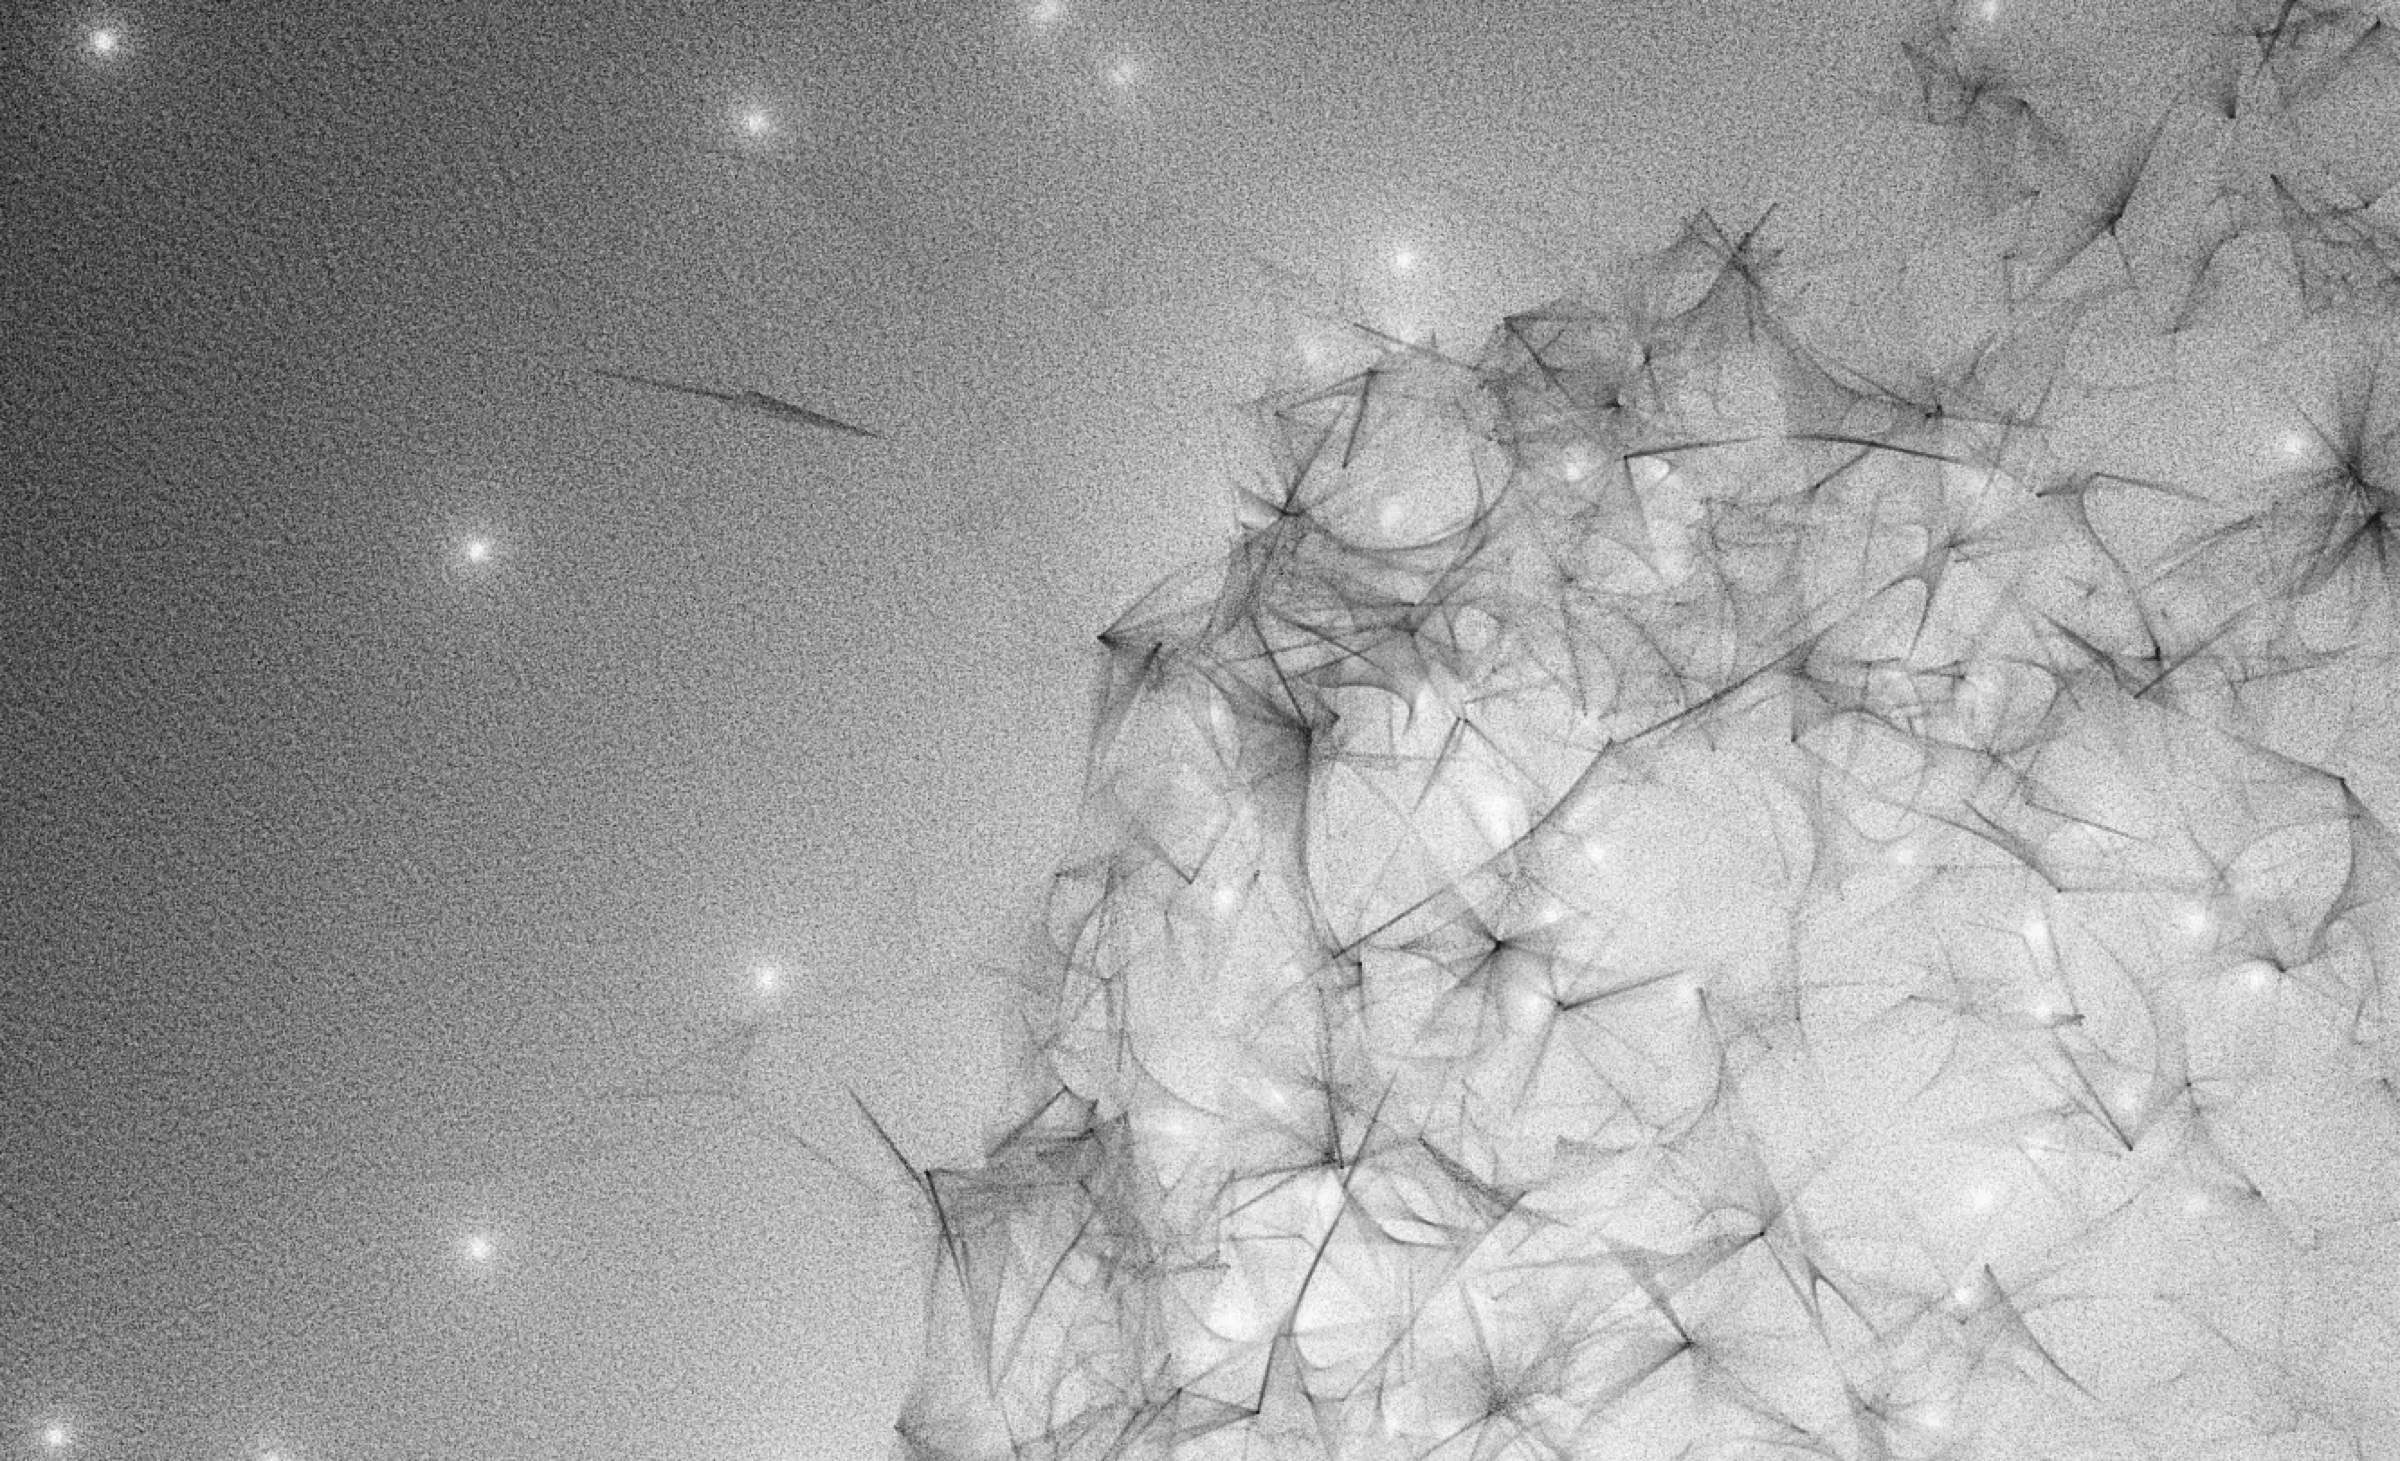
\includegraphics[width=\linewidth]{interp-4-2}\caption{detail.}\end{subfigure}
  \caption{\work{meetings are ripples}. Black lines between travellers are visible only where ripples from earlier meetings have lit the ground.}
  \label{fig:ripples}
\end{figure}

% ------------------------------------------------------------
\subsection{the collective fabric of age \& experience}
\label{sec:fabric}

\begin{interpretation}{\#5: the collective fabric of age \& experience}
  \item[thought] beings age and morph into more experienced beings over time. as they grow older, more beings are affected by their experience. we all live in the collective fabric of each other's experience.
  \item[expression] surround each being with a polygon. as they age, more nodes are added. therefore, younger ones are likely to be sharper; while older ones are likely to be rounder. as they age, expand the spread of the polygon \& move it closer to white. note that the size of the polygons are far greater than the size of the world.
  \item[parameters] population: 1000; day\_length: 48.
\end{interpretation}

\paragraph{Realisation.} Each being is surrounded by a polygon that begins as a rough triangle. Every year (every day of the world), it gains one to four nodes at random moments, each placed in one of the polygon's widest gaps, so a being of a hundred has some 250 nodes and is nearly a smooth curve. The nodes sit on a closed form of the being's own, a loop of noise that drifts slowly as the being ages, and each wanders a little off it. A polygon's size is its being's mass, times a factor that grows with age, times a personal \emph{impact} drawn log-normally, so that the old are likely to be large but some of the young are large and some of the old are small; at full size, polygons are several times larger than the world. The line is darker for the young and whiter for the old. The drawing accumulates.

\paragraph{What it shows.} No polygon can be seen whole; what is visible is their overlap (Figure~\ref{fig:fabric}). The young contribute sharp, dark, angular lines; the old, wide, pale, rounded ones. Because each polygon moves with its being, its routine is written across the whole picture, far from where the being actually is: every being's life is present everywhere, as a fold in a fabric of crumpled grey.

\anecdote{why this thought: someone older whose experience shaped yours, or the idea of a ``fabric'' of experience.}

\begin{figure}[t]
  \centering
  \begin{subfigure}[t]{0.49\linewidth}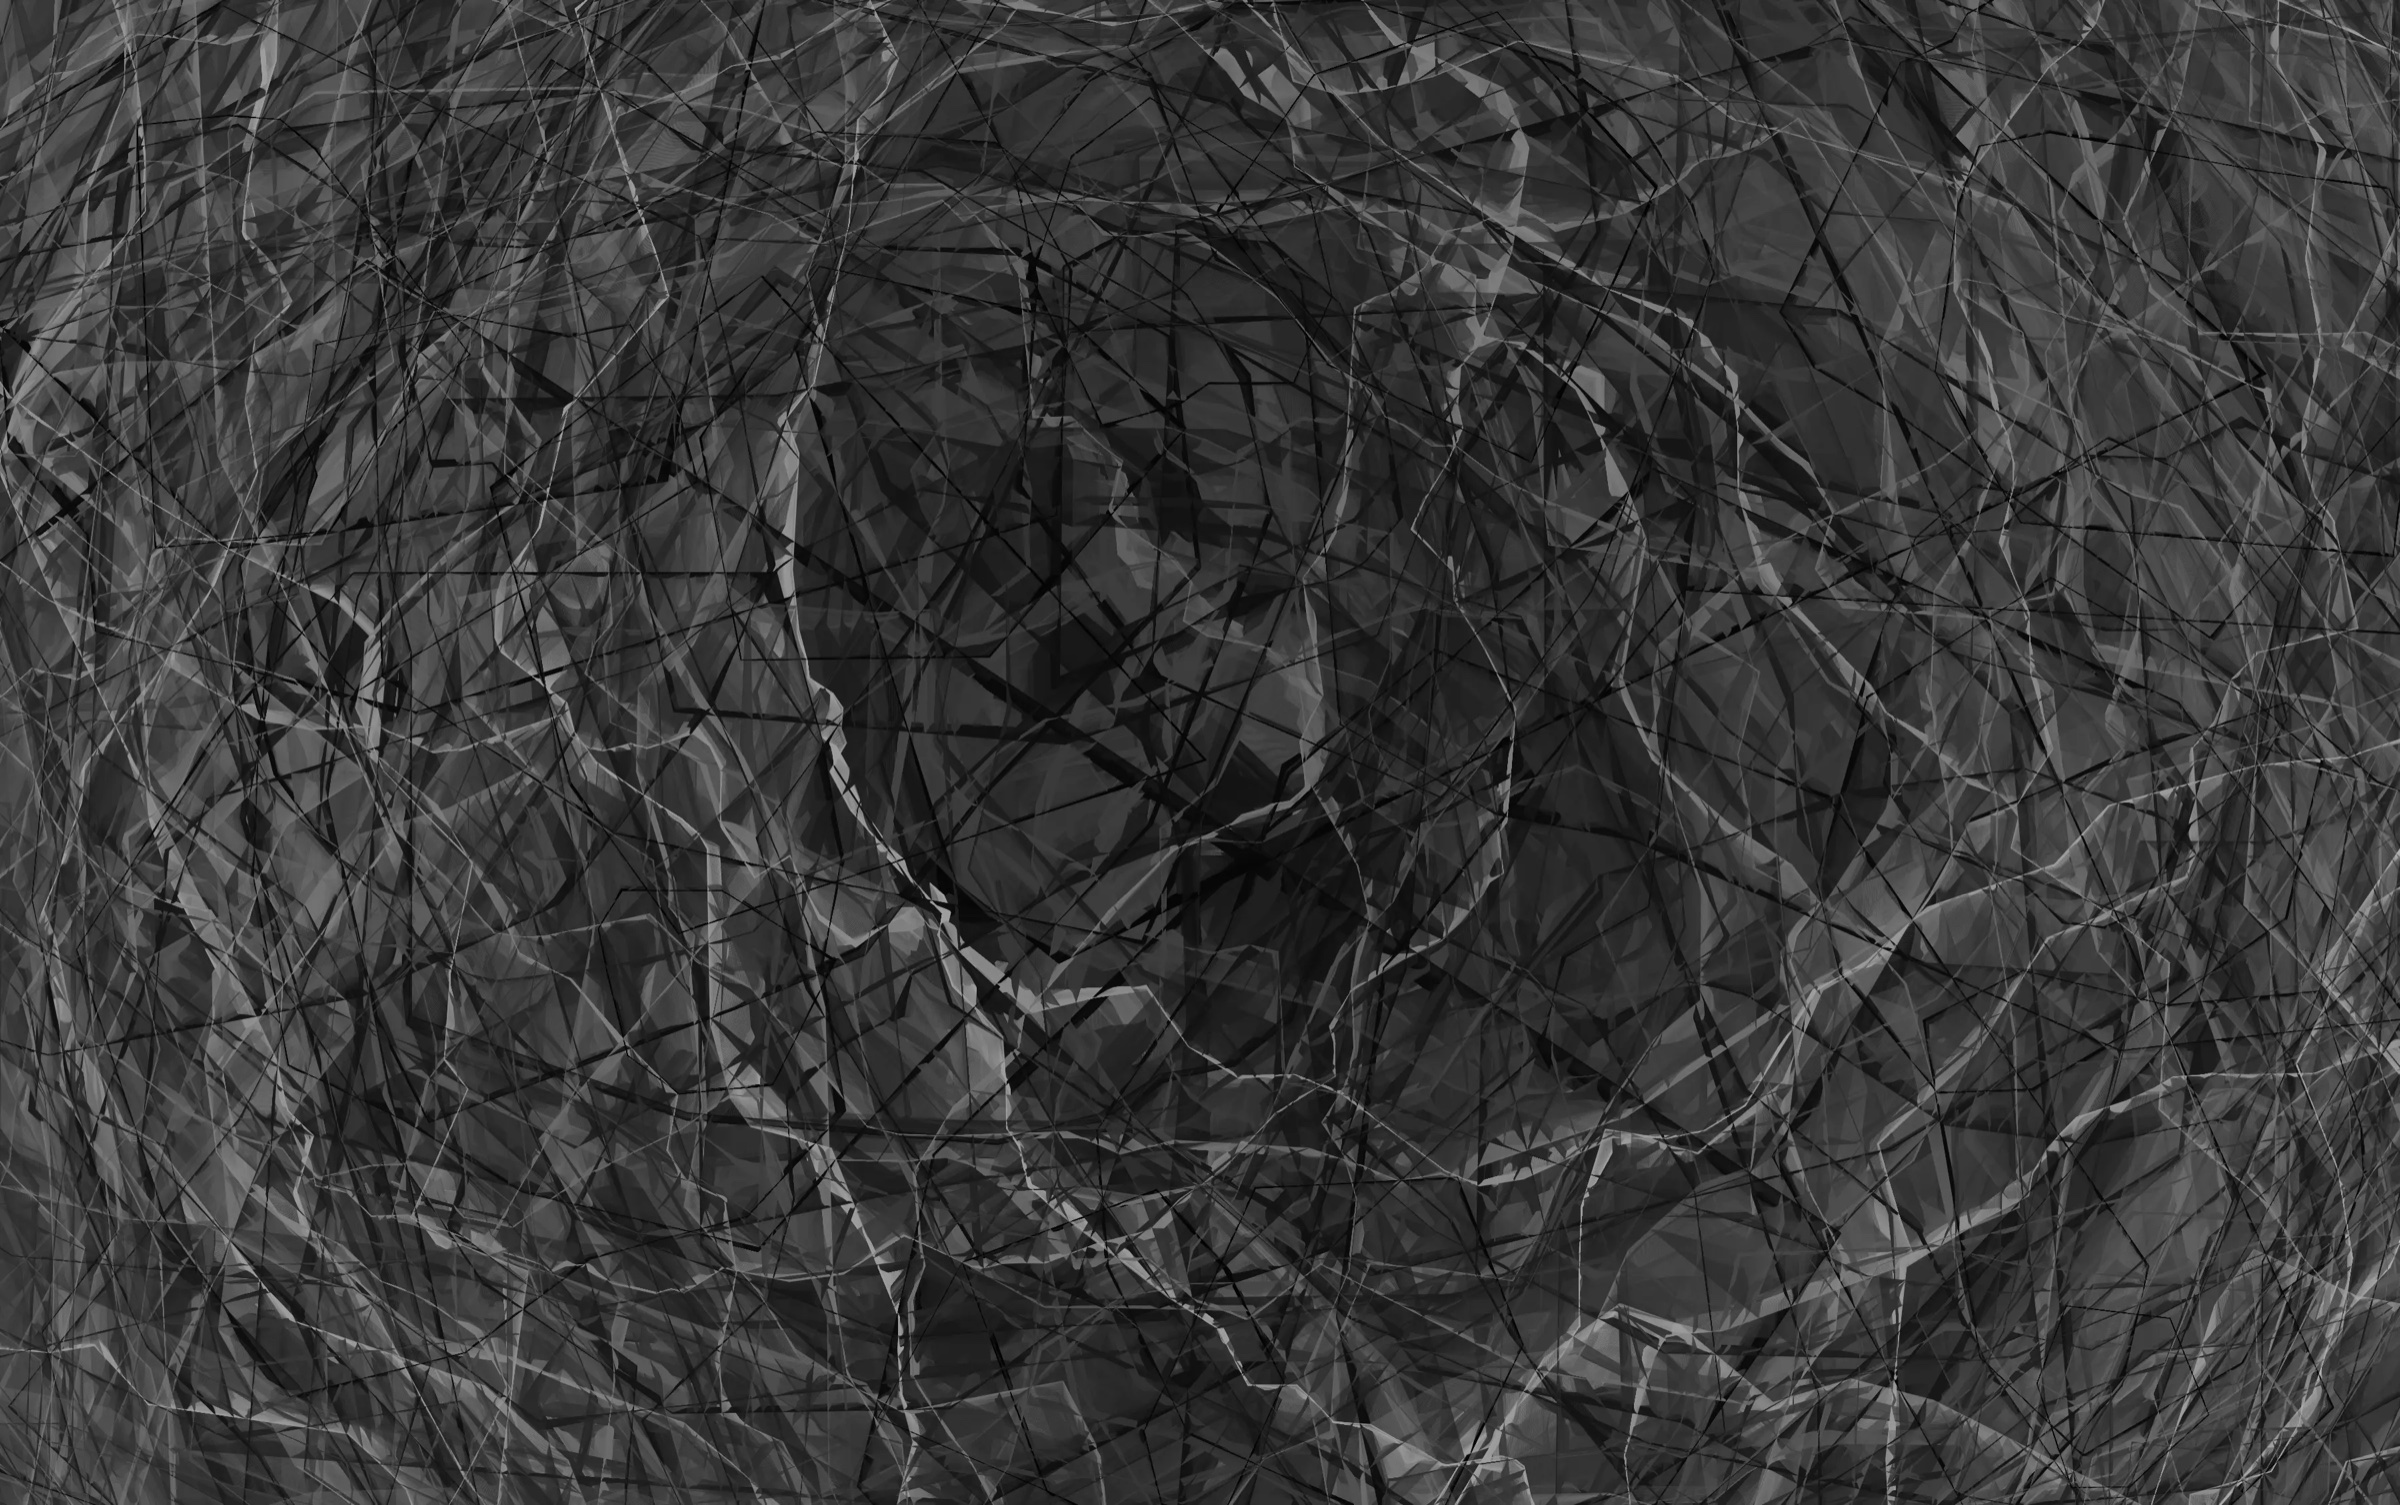
\includegraphics[width=\linewidth]{interp-5-1}\caption{}\end{subfigure}\hfill
  \begin{subfigure}[t]{0.49\linewidth}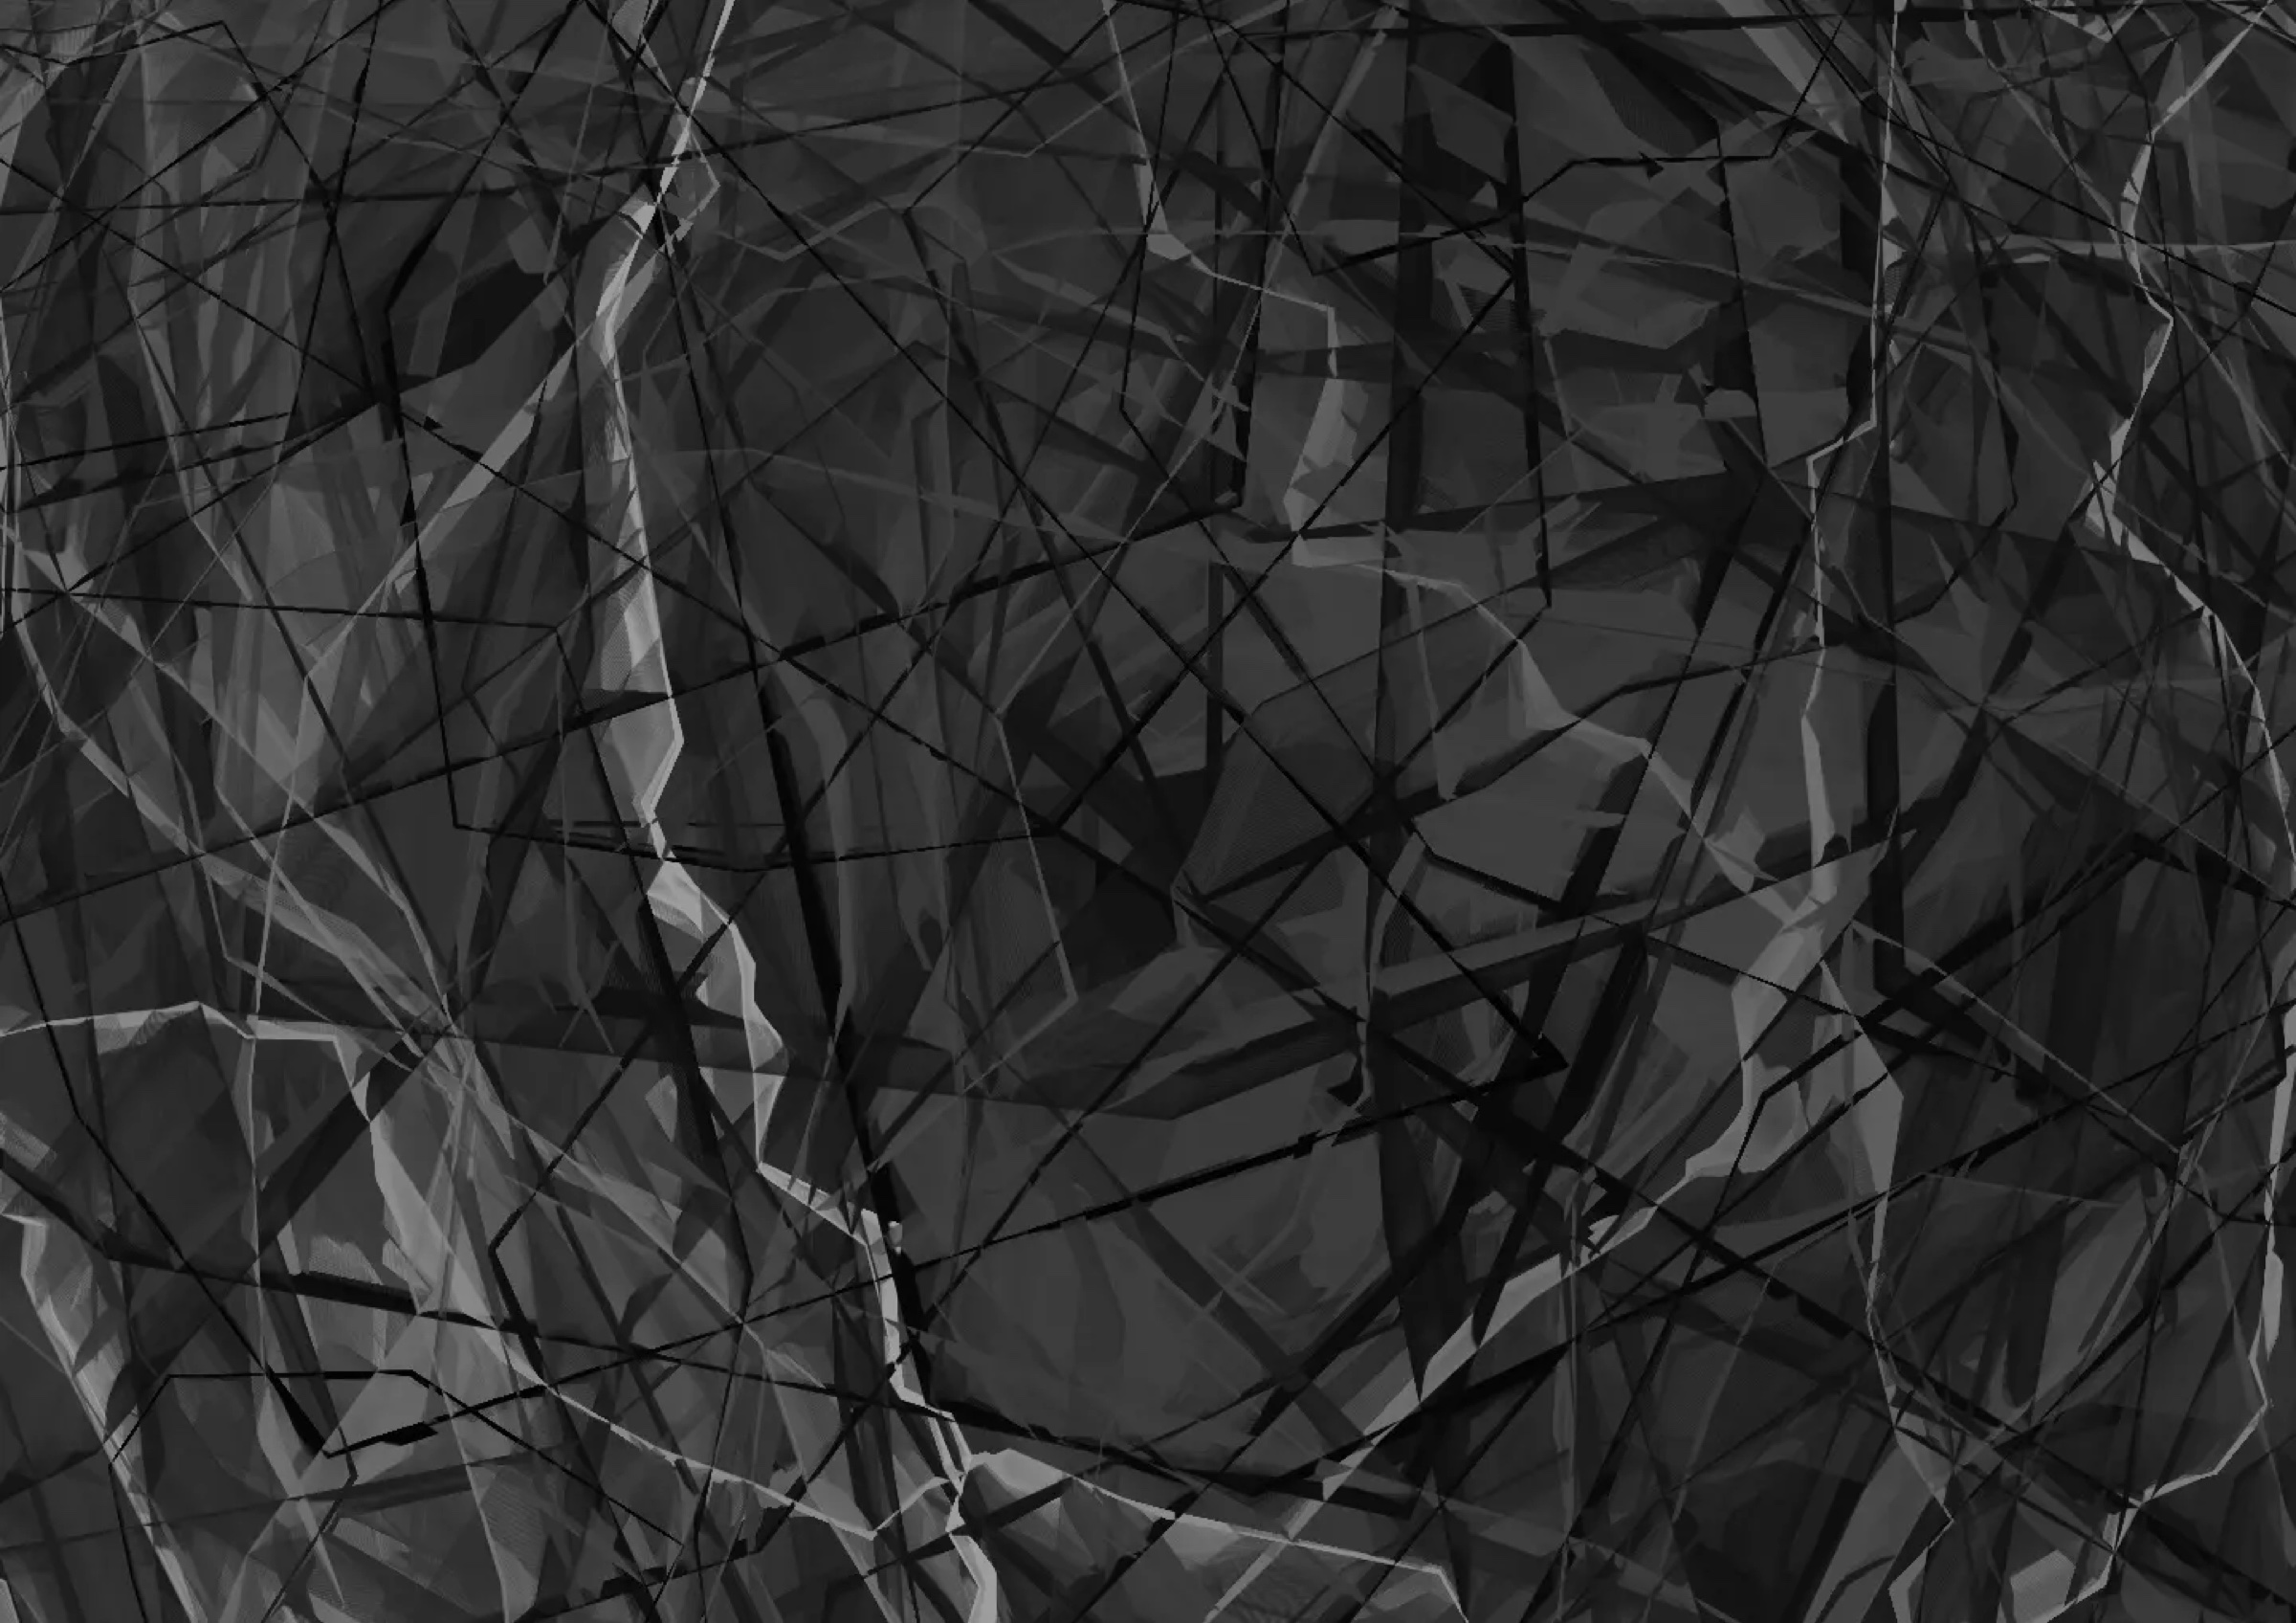
\includegraphics[width=\linewidth]{interp-5-2}\caption{detail.}\end{subfigure}
  \caption{\work{the collective fabric of age \& experience}. Polygons far larger than the world overlap into one surface: dark and sharp for the young, pale and rounded for the old.}
  \label{fig:fabric}
\end{figure}

% ------------------------------------------------------------
\subsection{separation}
\label{sec:separation}

\begin{interpretation}{\#6: separation}
  \item[thought] beings in different locations hold opposing views, and are separated over time.
  \item[expression] for each group of beings at a particular place, average out the direction that they arrived from, and treat it as an infinite line. for each of these lines, draw an orthogonal line between the place and its neighboring place in one of two colors. draw these lines over time.
  \item[parameters] population: 1000; day\_length: 48.
\end{interpretation}

\paragraph{Realisation.} Each place's surroundings are its eight nearest places. Every frame, the beings staying at each place are grouped by \emph{side}: the surrounding place that lies most in the direction from the place to the being. For each side, the beings' directions are averaged as lines rather than arrows, so that beings on opposite edges of a crowd agree instead of cancelling out. Each being on a side then draws its own line, orthogonal to that average, halfway between the place and the place on that side, each nudged by the being's own slowly drifting noise in position, tilt and thickness. Lines grow longer as the place grows more crowded, up to two and a half times the gap between the places. Each being is, at random and permanently, blue or red; colours are darkest at the centre of the world and lightest at its edge. Every line is faint, and strength comes only from how many lines pile up. The drawing accumulates.

\paragraph{What it shows.} Walls appear between neighbouring places, in the colours of the beings who stand on either side of them (Figure~\ref{fig:separation}). Busy places throw up long, dense barriers; quiet ones, short and faint ones. Again, the places themselves are never drawn, but the image organises itself around them as a field of starbursts, and the colour of each barrier records who happened to be standing there, over time.

\anecdote{why this thought: what prompted ``opposing views'' \& separation, & the choice of democrat blue \& republican red.}

\note{the expression says ``the direction that they arrived from''; the code averages the side of the place each staying being is on (close to where it arrived, but not the same). consider rewording the expression in the code header, & then here.}

\begin{figure}[t]
  \centering
  \begin{subfigure}[t]{0.49\linewidth}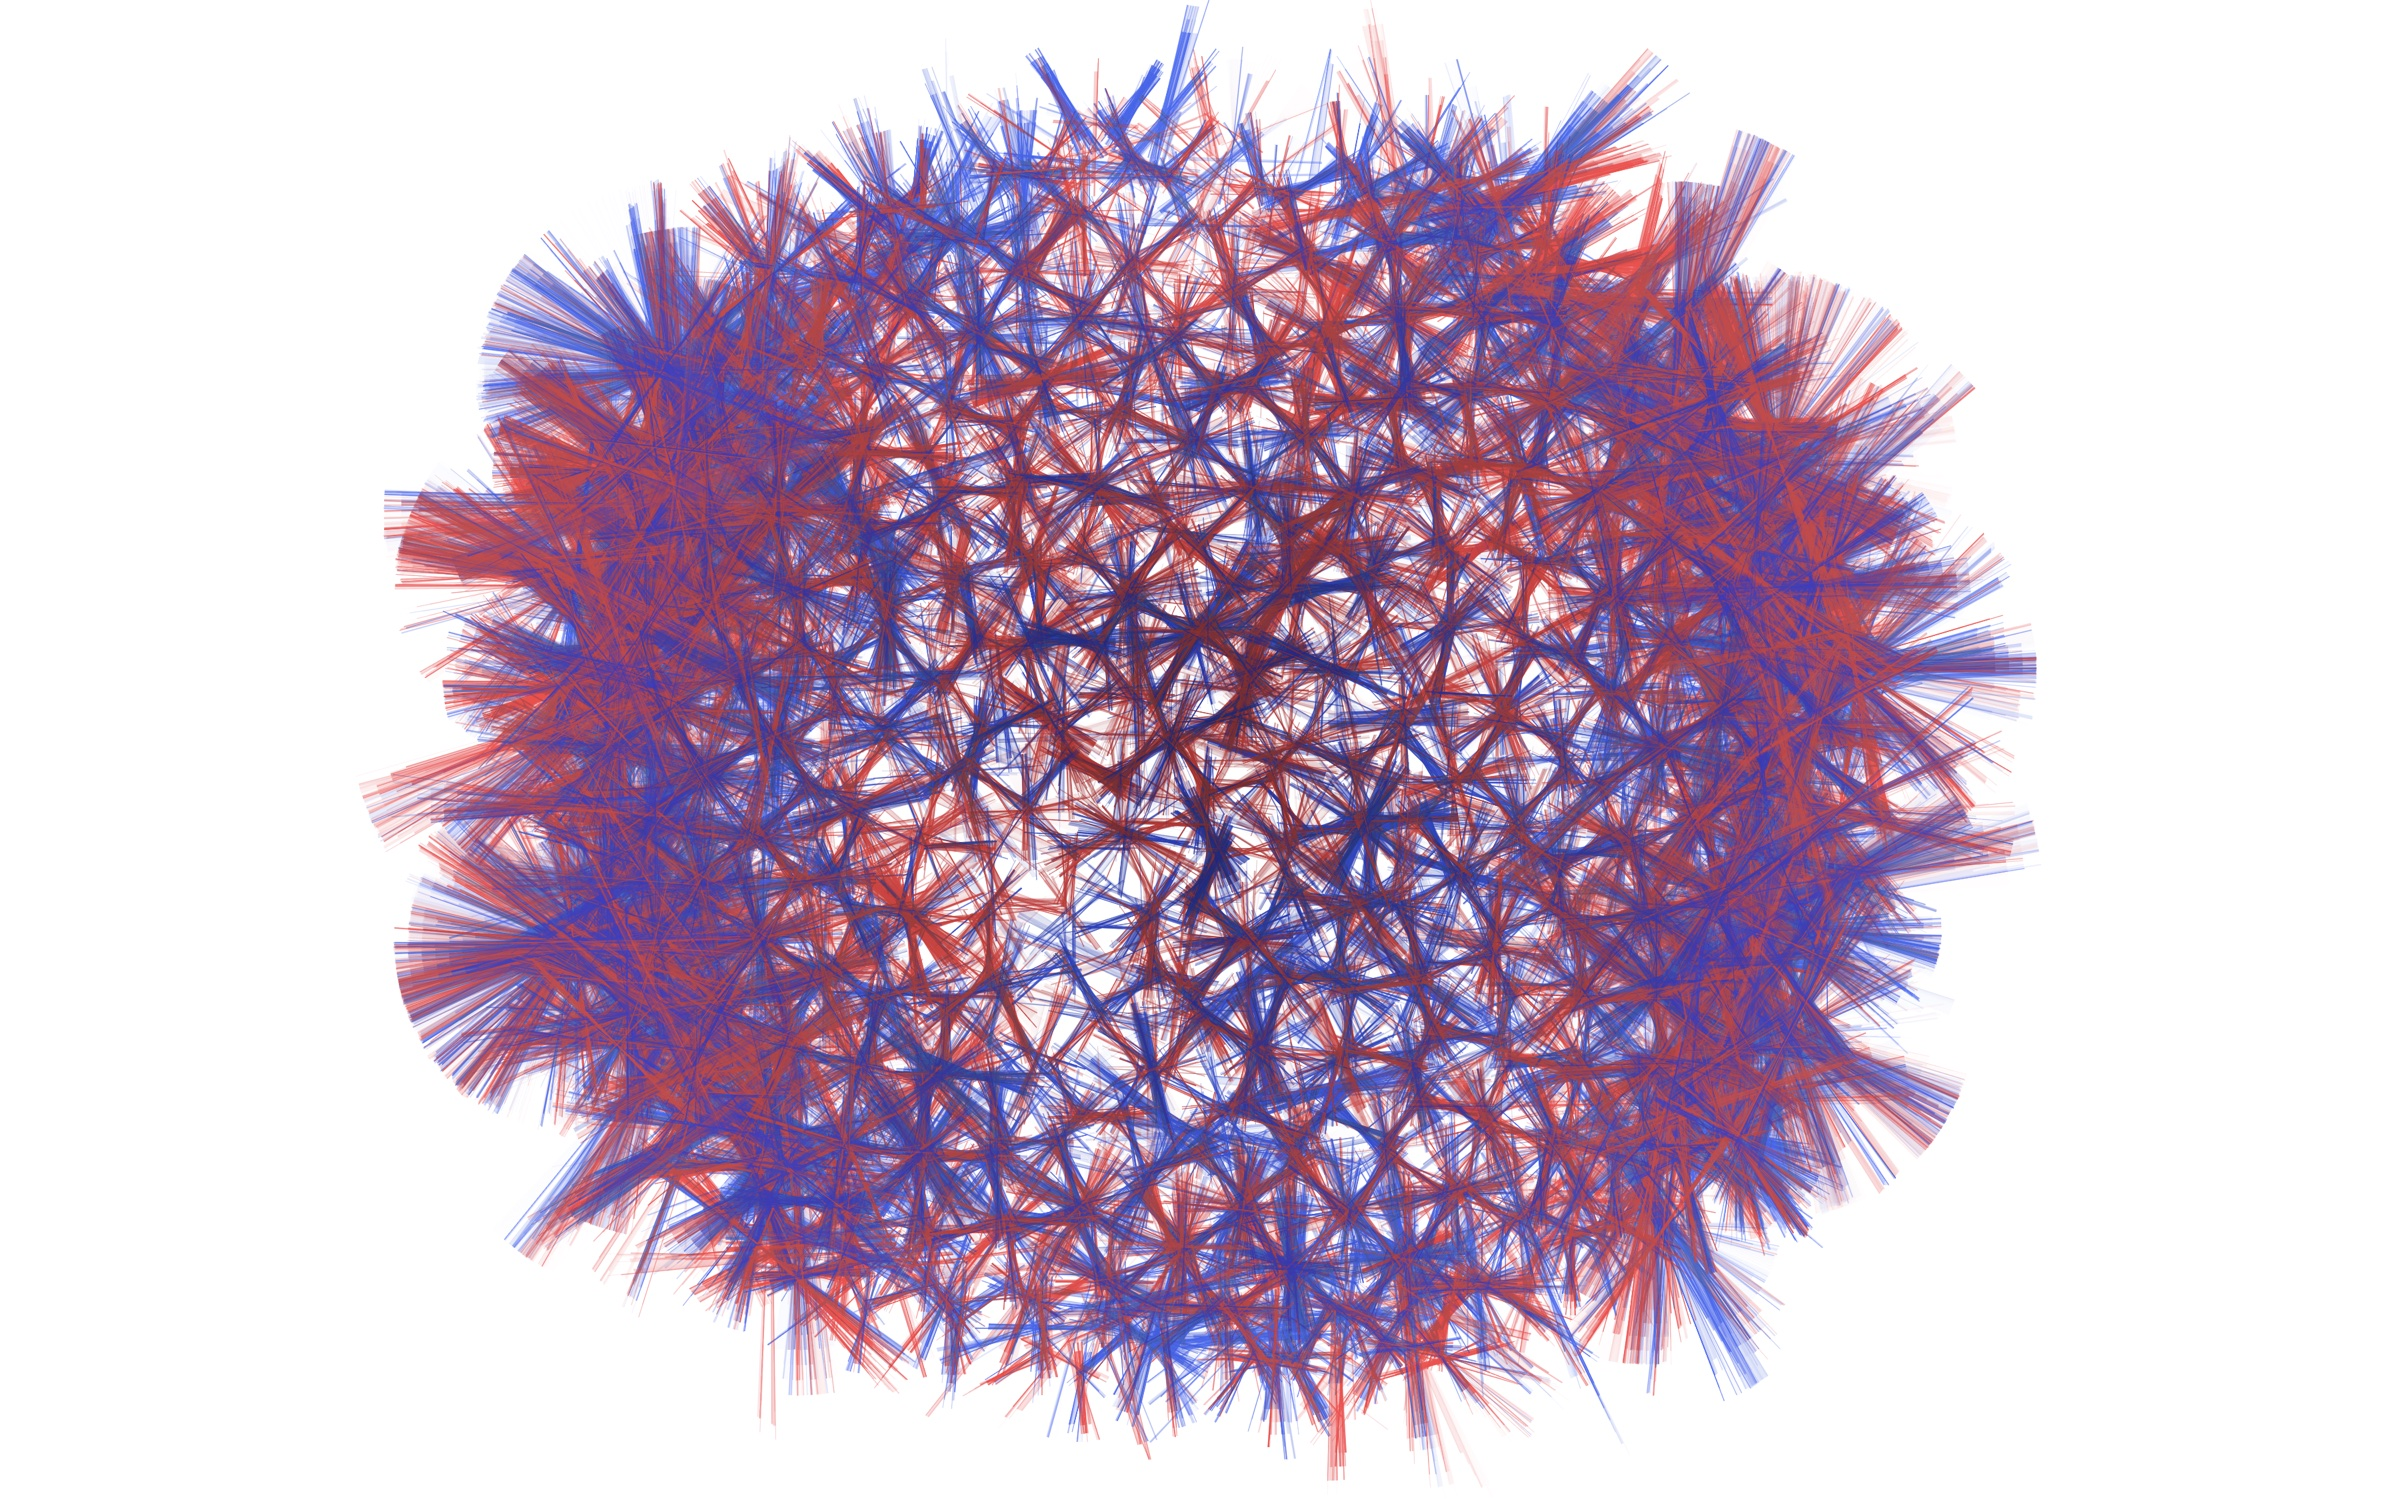
\includegraphics[width=\linewidth]{interp-6-1}\caption{}\end{subfigure}\hfill
  \begin{subfigure}[t]{0.49\linewidth}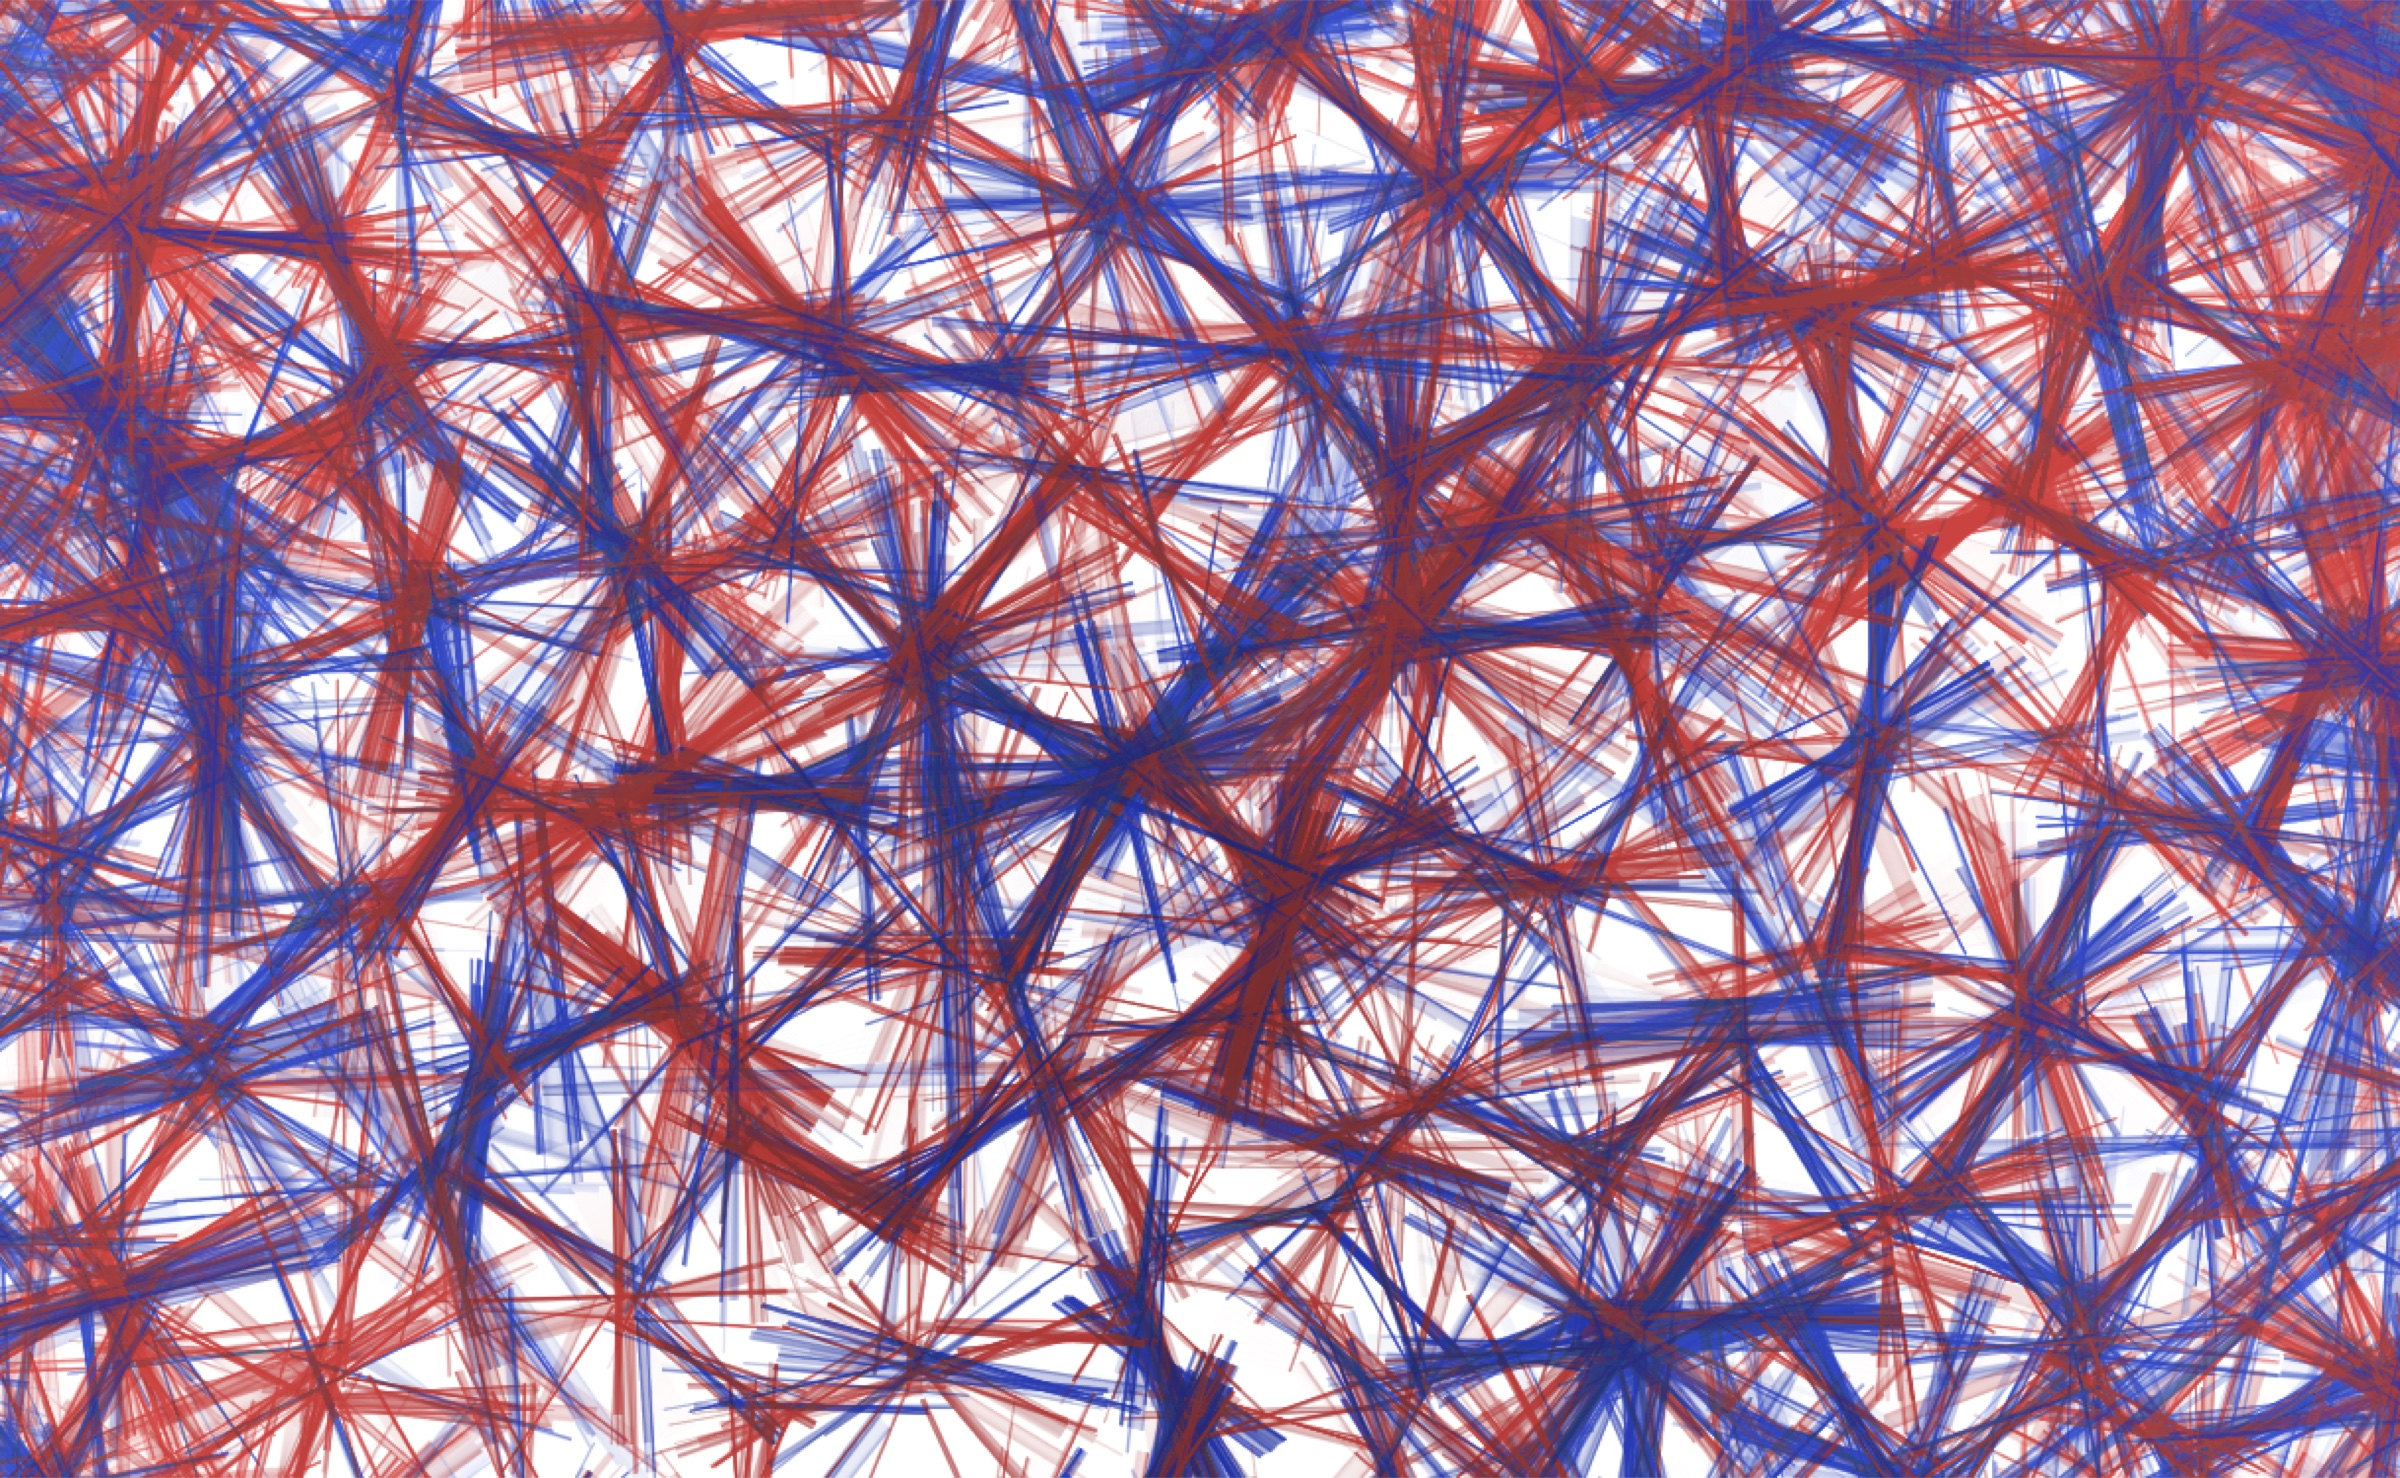
\includegraphics[width=\linewidth]{interp-6-2}\caption{detail.}\end{subfigure}
  \caption{\work{separation}. Lines are drawn between neighbouring places by the beings staying on either side; their colours are assigned at random.}
  \label{fig:separation}
\end{figure}

\section{Revising the Ground}
\label{sec:revision}

The base system described in Section~\ref{sec:system} is its second version. The first was written quickly, to get beings moving, and the first interpretations were made on it. When I began to measure it, rather than only watch it, I found that it did not do what its rules described, and that what interpretations could show was being decided by those failures rather than by their thoughts. This section reports that revision, because it bears on a claim that is easy to make and harder to keep: that an interpretation is a reading of a system's emergent behaviour.

\subsection{Measuring the system}

To compare the two versions, I built an analysis page that loads both systems' code unchanged, runs each in its own scope under the same conditions, and measures them through small adapters (Appendix~\ref{app:reproducibility}). It plots the underlying curves (energy, speed, places wished for and planned, the probability of dying), relationships between them, the simulation as lived (population, places reached a day, the share of beings travelling over time, age at death), a set of thirteen checks with a pass or fail for each system, and the main numbers across ten world set-ups. The comparison below is for a world of 1440$\times$900 pixels and 500 beings.

\subsection{What the first version did}

\begin{table}[t]
  \centering
  \small
  \begin{tabularx}{\linewidth}{@{}l X X@{}}
    \toprule
    & \textbf{first version} & \textbf{revised version} \\
    \midrule
    Destinations & any place in the world, at random (about 400\,px away on average) & a loop of nearby places, chosen at the being's own range \\
    Beings travelling at any moment & about 98\% & about 28--35\% \\
    Departures & bunched on the hour (23\% in the busiest 1\% of moments) & spread evenly (1.9\% in the busiest 1\%) \\
    18--45-year-olds reaching no place in a day & 36--38\% & 0.1\% \\
    Planned slots & about 4, whatever the age & about 11 / 4 / 2 for ages 18--35 / 36--59 / 60+ \\
    Death roll & every frame of the killing hour, until the population fell to 95\% & once a day, per being \\
    Lifespans & nobody past their late forties & median 62--78 by vigor; about 7\% reach 100 \\
    Re-planning & everyone at once, at midnight & each being at its own day start \\
    \bottomrule
  \end{tabularx}
  \caption{The first and revised base systems, measured under the same conditions. The first-version numbers are for 5-hour days, the setting it was used with.}
  \label{tab:revision}
  \note{the revised-version column mixes measurements from 24-hour days (after the day-length change) & the first version's from 5-hour days. that's fair (each in the setting it was used in), but say it plainly, as the caption does, or re-measure both at one setting.}
\end{table}

Table~\ref{tab:revision} summarises the differences. In the first version, a being chose its destinations at random from the whole world, and walked to them at a speed that, for an adult, was about one pixel a frame. A typical trip was longer than a day, and a being chose its next destination only once it had arrived, so nearly every being was travelling at every moment, and more than a third of young adults reached no place at all in a day. Departures happened only when the world's hour matched a slot, so beings left in waves on the hour. Days that were short on screen also ran out of hours: slots past the end of the day were never reached, so everyone planned about four slots regardless of age, and the age-dependent busyness the system was meant to have was never expressed. The death roll was repeated on every frame of the killing hour until the population fell below its threshold; births refilled it and the roll culled it again, so about four times as many beings died as should have, and nobody lived past their late forties. Every birthday fell on the same frame, so everyone re-planned at once.

None of these behaviours was intended, and none was visible as a bug: the world looked lively, and beings moved. But each changed what the interpretations drew. With nearly everyone always travelling, a reading of passing such as \work{missed connections} had almost no staying to set it against. With crowds rarely reaching places, a mesh has few still points to gather around. And with nobody old, a reading of ageing such as \work{the collective fabric}, made after the revision, would have had nothing to read. The first interpretations, made on the first version, were to a real extent readings of its defects.
\note{check: which interpretations (by version number) were first made on the old system. the talk notes of 6 august show 1.5, 2.0, 3.0 \& 4.1.}

\subsection{The case of home}

One revision went the other way. During the rework I added a \emph{home}: each being's routine began and ended at a fixed place, the way many human days do. It seemed a natural rule from life. Measured over 400 days, however, it produced a strong, unplanned emergent pattern. Newborns appear beside their parents, and so take homes near their parents' homes; over generations, homes clustered, until 67 of 125 places went unused and the busiest place held eight times the average crowd. The world slowly emptied into a few neighbourhoods. Removing home, so that each new routine starts wherever the being is, dissolved the clustering (at most 7 places unused, and the busiest three to four times the average), and also reduced the share of beings travelling, since a day no longer began with a walk home.

This is emergence in exactly Bar-Yam's sense: two individually reasonable rules (a fixed home; children born beside their parents) combining into a collective outcome that neither specifies~\cite{baryam1997}. It is also an outcome that would have dominated every interpretation drawn from the world. I removed home not because the clustering was uninteresting (it may well be the subject of a future interpretation) but because it was not a rule I had chosen to make, and the base system's job is to be a ground, not a thesis.

\subsection{What the revision shows}

The lesson I draw is a methodological one. The interpretations are presented as readings of a system's emergent behaviour, and the reading is where the artist's voice lies. But the ground on which they stand is not neutral, and its accidents read as content: a viewer cannot tell a defect in the ground from a choice in the reading. For an artist working this way, measuring the base system, with its ranges as well as its averages, is part of the work, not a step before it.

\section{Discussion}
\label{sec:discussion}

\subsection{What everyday rules afford}

The central claim of this work is that rules drawn from everyday life change what emergence can mean in an artwork. Three things support it.

First, everyday rules give interpretations something to be \emph{about}. A thought such as ``we walk by so many people'' can be tested against a system in which beings really do walk by each other, on their way between places they really do frequent. The same thought, read against Reas's elements or against a cellular automaton, would be a metaphor laid over an abstraction. Here it is a reading of a world that already contains walking, passing and staying.

Second, everyday rules make the system's emergent structure recognisable. The places in Section~\ref{sec:interpretations} are never drawn, yet three of the six interpretations reveal them, as the stars of a mesh, the bright fields of ripples and the centres of the separation's starbursts. This is not because the interpretations look for places, but because routines make beings return, and returning is what everyday life is mostly made of~\cite{gonzalez2008, song2010}. The interpretations converge on the structure of the system without being told it.

Third, everyday rules let a single system carry readings that are personal and still grounded. Each of the six thoughts comes from my own experience, and none of them was written to suit the system. That they can all be drawn from it suggests that a system made from life, even one as simple as this, holds more of life than its rules state, which is the promise of emergence in the first place.

\subsection{The interpretation as authorship}

In instruction art, the instruction belongs to the artist and its execution to someone else~\cite{lewitt1967, ono1964, obrist2013}. In this work both belong to me, yet the thought and the expression are still distinct, and the distance between them is where the work's judgements are made. Many interpretations went through several expressions before one matched its thought (the source tree keeps every earlier version), and in most cases it was the thought that held still.\note{check this against \code{wip/}: did the thoughts stay the same across versions while the expressions changed? if not, say what changed.} The three-part format is, in this sense, less a description of a finished work than a discipline for making one, and it is a format other artists can take up with other systems, or indeed with this one.

\subsection{Reading division into a neutral world}

\work{separation} deserves a separate comment, because it makes a claim that the system does not. Its thought speaks of beings that ``hold opposing views'', but beings in this system hold no views at all. Their colours are assigned at random, and they choose places without regard to anyone's colour. This is the opposite of Schelling's model of segregation, in which mild individual preferences about one's neighbours produce stark division~\cite{schelling1971}. In \work{separation}, there are no preferences, and the division is drawn entirely by the reader.

I think this is the interpretation's point rather than its weakness. The image looks like a map of a divided world, and it is made from beings who keep ordinary routines and have no opinions about each other. It asks how much of the division we see in maps of real places is in the people, and how much is in the reading.

\subsection{Limitations}

\paragraph{Not a model of a city.} The system is inspired by everyday life in New York, but it is not calibrated against any data, and it does not reproduce any measured property of real mobility. Places lie on a regular spiral, not a street network; a day is a year; there are no homes, no work, no weekends, no relationships, and no inheritance. Its rules are recognisable as life, not representative of it, and the claims made here are claims about an artwork.

\paragraph{Emergence, claimed qualitatively.} The emergent properties reported in Sections~\ref{sec:system} and~\ref{sec:revision} (a steady flow, neighbourhoods without homes, clustering with them) are measured, but the claims about what the interpretations reveal are made by looking. I have not measured, for instance, how closely the stars of the mesh coincide with places.

\paragraph{One artist.} All six interpretations are by the system's author. The claim that the format separates the maker of a system from its reader would be stronger if others read the same system; this is an invitation as much as a limitation (Section~\ref{sec:conclusion}).

\paragraph{Parameters as a confound.} Interpretations run in worlds of different sizes, densities and speeds. The rules are the same, but the worlds are not, and some differences between images come from their parameters rather than their readings.

\section{Conclusion and Future Work}
\label{sec:conclusion}

This paper has presented \emph{emergence-study}, an artwork in which a simulated world built from the rules of everyday life is never shown, and is seen only through software-interpretations: thoughts written in English from lived experience and realised as algorithms that read the world. I have described the base system in full, the three-part format of thought, expression and parameters, and six interpretations made with it, and I have reported how measuring and revising the base system changed what those interpretations could show.

Two directions follow. The first is to open the system to other readers. Because the interface is narrow and the format is plain, other artists can write interpretations of the same world, and a body of readings by many people would test whether one system of everyday rules can hold as many readings as I hope. The second is to keep the ground honest as it grows: to add rules only where life suggests them, and to measure what each one does to the world before reading it. Some of what such measurement uncovers, like the neighbourhoods that homes produced, may become interpretations in their own right.

\identifying{The system, the interpretations and the analysis pages are open source at \url{https://github.com/arjunmakesthings}.\note{put the exact repository link here.}}{The system, the interpretations and the analysis pages are open source; the link is withheld for review.}


\ifanonymous\else
  \section*{Acknowledgments}

This work began during a batch at the Recurse Center in the summer of 2026; I am grateful to the programmers I met and worked with there. I also thank the Interactive Telecommunications Program at New York University, and the audience of Processing Community Day New York 2026, where the work was first presented.
\note{add anyone who helped: recursers, itp faculty, peers. check the pcd date/name.}

\fi

\bibliographystyle{plainnat}
\bibliography{references}

\appendix
\section{The Rules in Full}
\label{app:rules}

Notation: $N_0$ is the starting population, $W \times H$ the world's size, $D$ the day length (seconds on screen per day), and $M$ the maximum mass. $\mathcal{N}(\mu, \sigma)$ is a normal draw, $\mathcal{U}(a, b)$ a uniform draw, $\sigma(x) = 1/(1+e^{-x})$ the logistic function, and $\mathrm{clamp}(x, a, b)$ limits $x$ to $[a, b]$. Ages $a$ are in years; one day of the world is one year.

\subsection*{World}
\begin{align*}
  \text{places:}\quad & n = \max\!\big(2, \lfloor N_0/4 \rfloor\big), \qquad R = 0.45\,\min(W, H) \\
  \text{place } i:\quad & r_i = R\sqrt{(i + 0.5)/n}, \qquad \theta_i = i\,\pi(3 - \sqrt{5}) \\
  \text{place spacing:}\quad & s = R\sqrt{\pi / n} \\
  \text{frames per hour:}\quad & h = 60D / 24 \\
  \text{pace (px per frame at full energy):}\quad & v_0 = s / (0.75\,h) \\
  \text{place radius, with crowd } c:\quad & \tfrac{M}{2}\sqrt{c/0.9} + M \\
  \text{starting ages:}\quad & a = \mathrm{round}\big(\mathrm{clamp}(\mathcal{N}(32, 18), 0, 80)\big)
\end{align*}

\subsection*{Traits (per being, not inherited)}
\begin{align*}
  m_{\max} &= \mathrm{clamp}\big(\lfloor \mathcal{N}(10, 6) \rfloor, \min(5, M), M\big), \qquad a_m = \lfloor \mathcal{N}(18, 1) \rfloor \\
  u &\sim \mathcal{U}(0.75, 1.25) \quad \text{(walking pace)} \\
  \nu &= e^{\mathcal{N}(0,\, 0.2)} \quad \text{(vigor)} \\
  \rho &= s\, e^{\mathcal{N}(0.4,\, 0.6)} \quad \text{(range)}
\end{align*}

\subsection*{Body over age}
\begin{align*}
  m(a) &= m_{\max}\,\frac{1 - e^{-5a/a_m}}{1 - e^{-5}} \\
  E(a) &= 10\,\nu\;\sigma\!\Big(\frac{a - 12}{3}\Big)\Big(0.2 + 0.8\,\sigma\!\Big(\!-\frac{a - 50}{7}\Big)\Big) \\
  v(a) &= v_0\,\frac{E(a)}{10}\,u \quad \text{(speed, px per frame)}
\end{align*}

\subsection*{Routine}
\begin{align*}
  g(a) &= e^{-(a - 25)^2 / (2 \cdot 10^2)} \\
  \text{busyness:}\quad b &= \mathrm{clamp}\Big(\mathrm{round}\big(\mathcal{N}\big(2 + 10\,g(a),\; 1.25 + 3.5\,(1 - g(a))\big)\big), 2, 12\Big) \\
  \Pr(\text{next place } p \mid \text{last place } q) &\propto e^{-\lVert p - q \rVert / \rho}, \quad \text{over places that still close the loop within 24 hours}
\end{align*}
Each slot lasts the trip to its place plus a minimum stay of 1 hour; spare hours are divided by random shares among the slots. Routines are renewed on birthdays with probability 1 (ages 2--6), 0.5 (7--60) or 0.25 (over 60), and otherwise re-timed; the new plan takes effect at the being's own day start. Beings under 2 do not move.

\subsection*{Birth and death}
\begin{align*}
  \Pr(\text{death today}) &= \Big(0.0002 + 0.12\,\min(a/100, 1)^3\Big)\,\frac{1}{\nu^2}, \quad \text{rolled once a day, if } N > 0.95\,N_0 \\
  \Pr(\text{child}) &= 0.2\;\sigma\!\Big(\frac{a - 18}{2}\Big)\,\sigma\!\Big(\!-\frac{a - 40}{2}\Big), \quad \text{while } N < N_0,\ \text{both parents aged } 18\text{--}45 \text{ and neighbours}
\end{align*}
Neighbours are beings within $2M$. Each pair has at most one child per round; the newborn appears at the midpoint of its parents. Overlapping beings are pushed apart symmetrically, in two passes over a spatial grid, every frame.

\section{Reproducibility}
\label{app:reproducibility}

The system is written in JavaScript with p5.js~1.11, in two files (\code{world.js}, \code{being.js}), and runs in any modern browser with no build step. Each interpretation is a single file that creates a world, runs it every frame, and draws from it; switching between interpretations means loading a different file.

The measurements in Sections~\ref{sec:system} and~\ref{sec:revision} were made headlessly, by running the unmodified \code{World} and \code{Being} classes in Node.js with a minimal stand-in for the parts of p5.js they use (vectors, random draws, and constraint), and instrumenting them from outside. The analysis pages that produced Figure~\ref{fig:graphs} and Table~\ref{tab:revision} run both versions of the system side by side, unchanged, each through a small adapter that says how its beings are measured; they are included in the repository. Unless stated otherwise, measurements are for a world of 1440$\times$900 pixels and 500 beings.
\note{say which commit the paper describes (e.g. a git tag like \code{paper-v1}), so reviewers can run exactly this version.}


\end{document}
